%----------------------------------------------------------------------------
\appendix
%----------------------------------------------------------------------------
\chapter*{\fuggelek}\addcontentsline{toc}{chapter}{\fuggelek}
\setcounter{chapter}{\appendixnumber}
%\setcounter{equation}{6} % a fofejezet-szamlalo az angol ABC 6. betuje (F) lesz
\numberwithin{equation}{section}
\numberwithin{figure}{section}
\numberwithin{lstlisting}{section}
%\numberwithin{tabular}{section}

%----------------------------------------------------------------------------
\section{Pictures of Demonstrator railway system} \label{appendix:HWPictures}
%----------------------------------------------------------------------------
\begin{figure}[H]
	\centering
	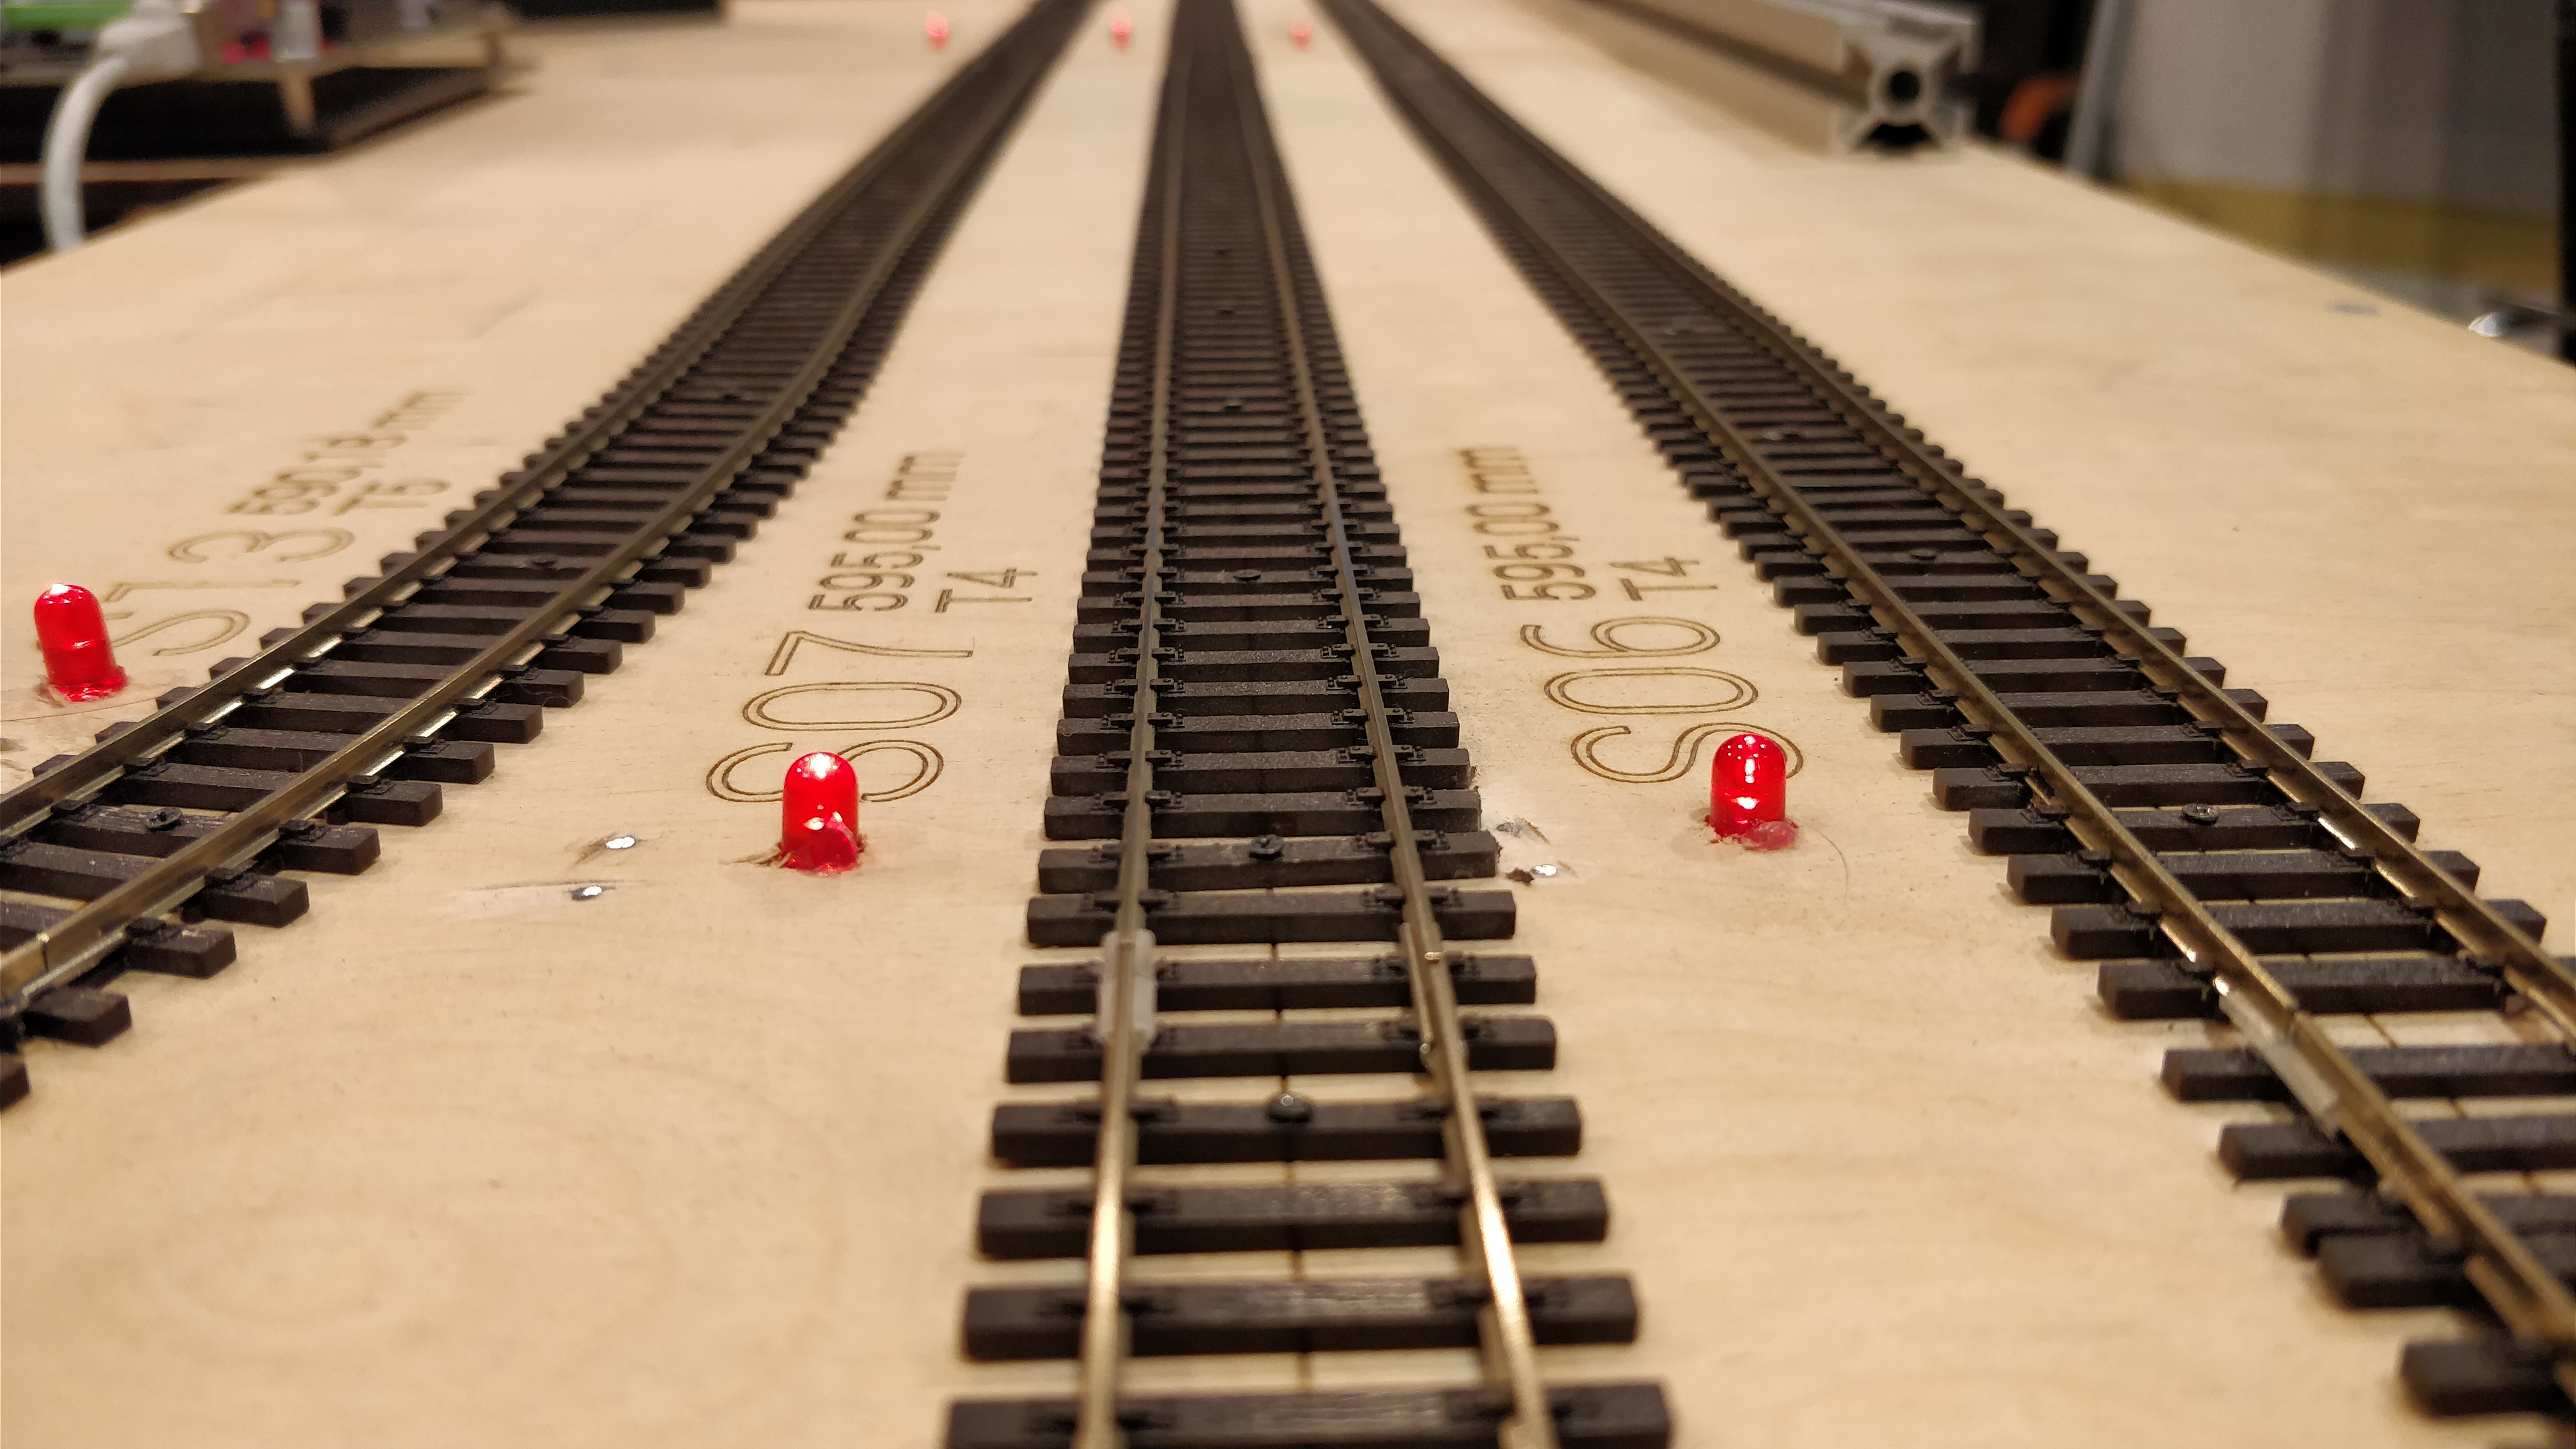
\includegraphics[width=150mm, keepaspectratio]{figures/modes3/section.jpg}
	\caption{Railway Section}
	\label{fig:section}
\end{figure}
%
%\begin{figure}[!h]
%	\centering
%	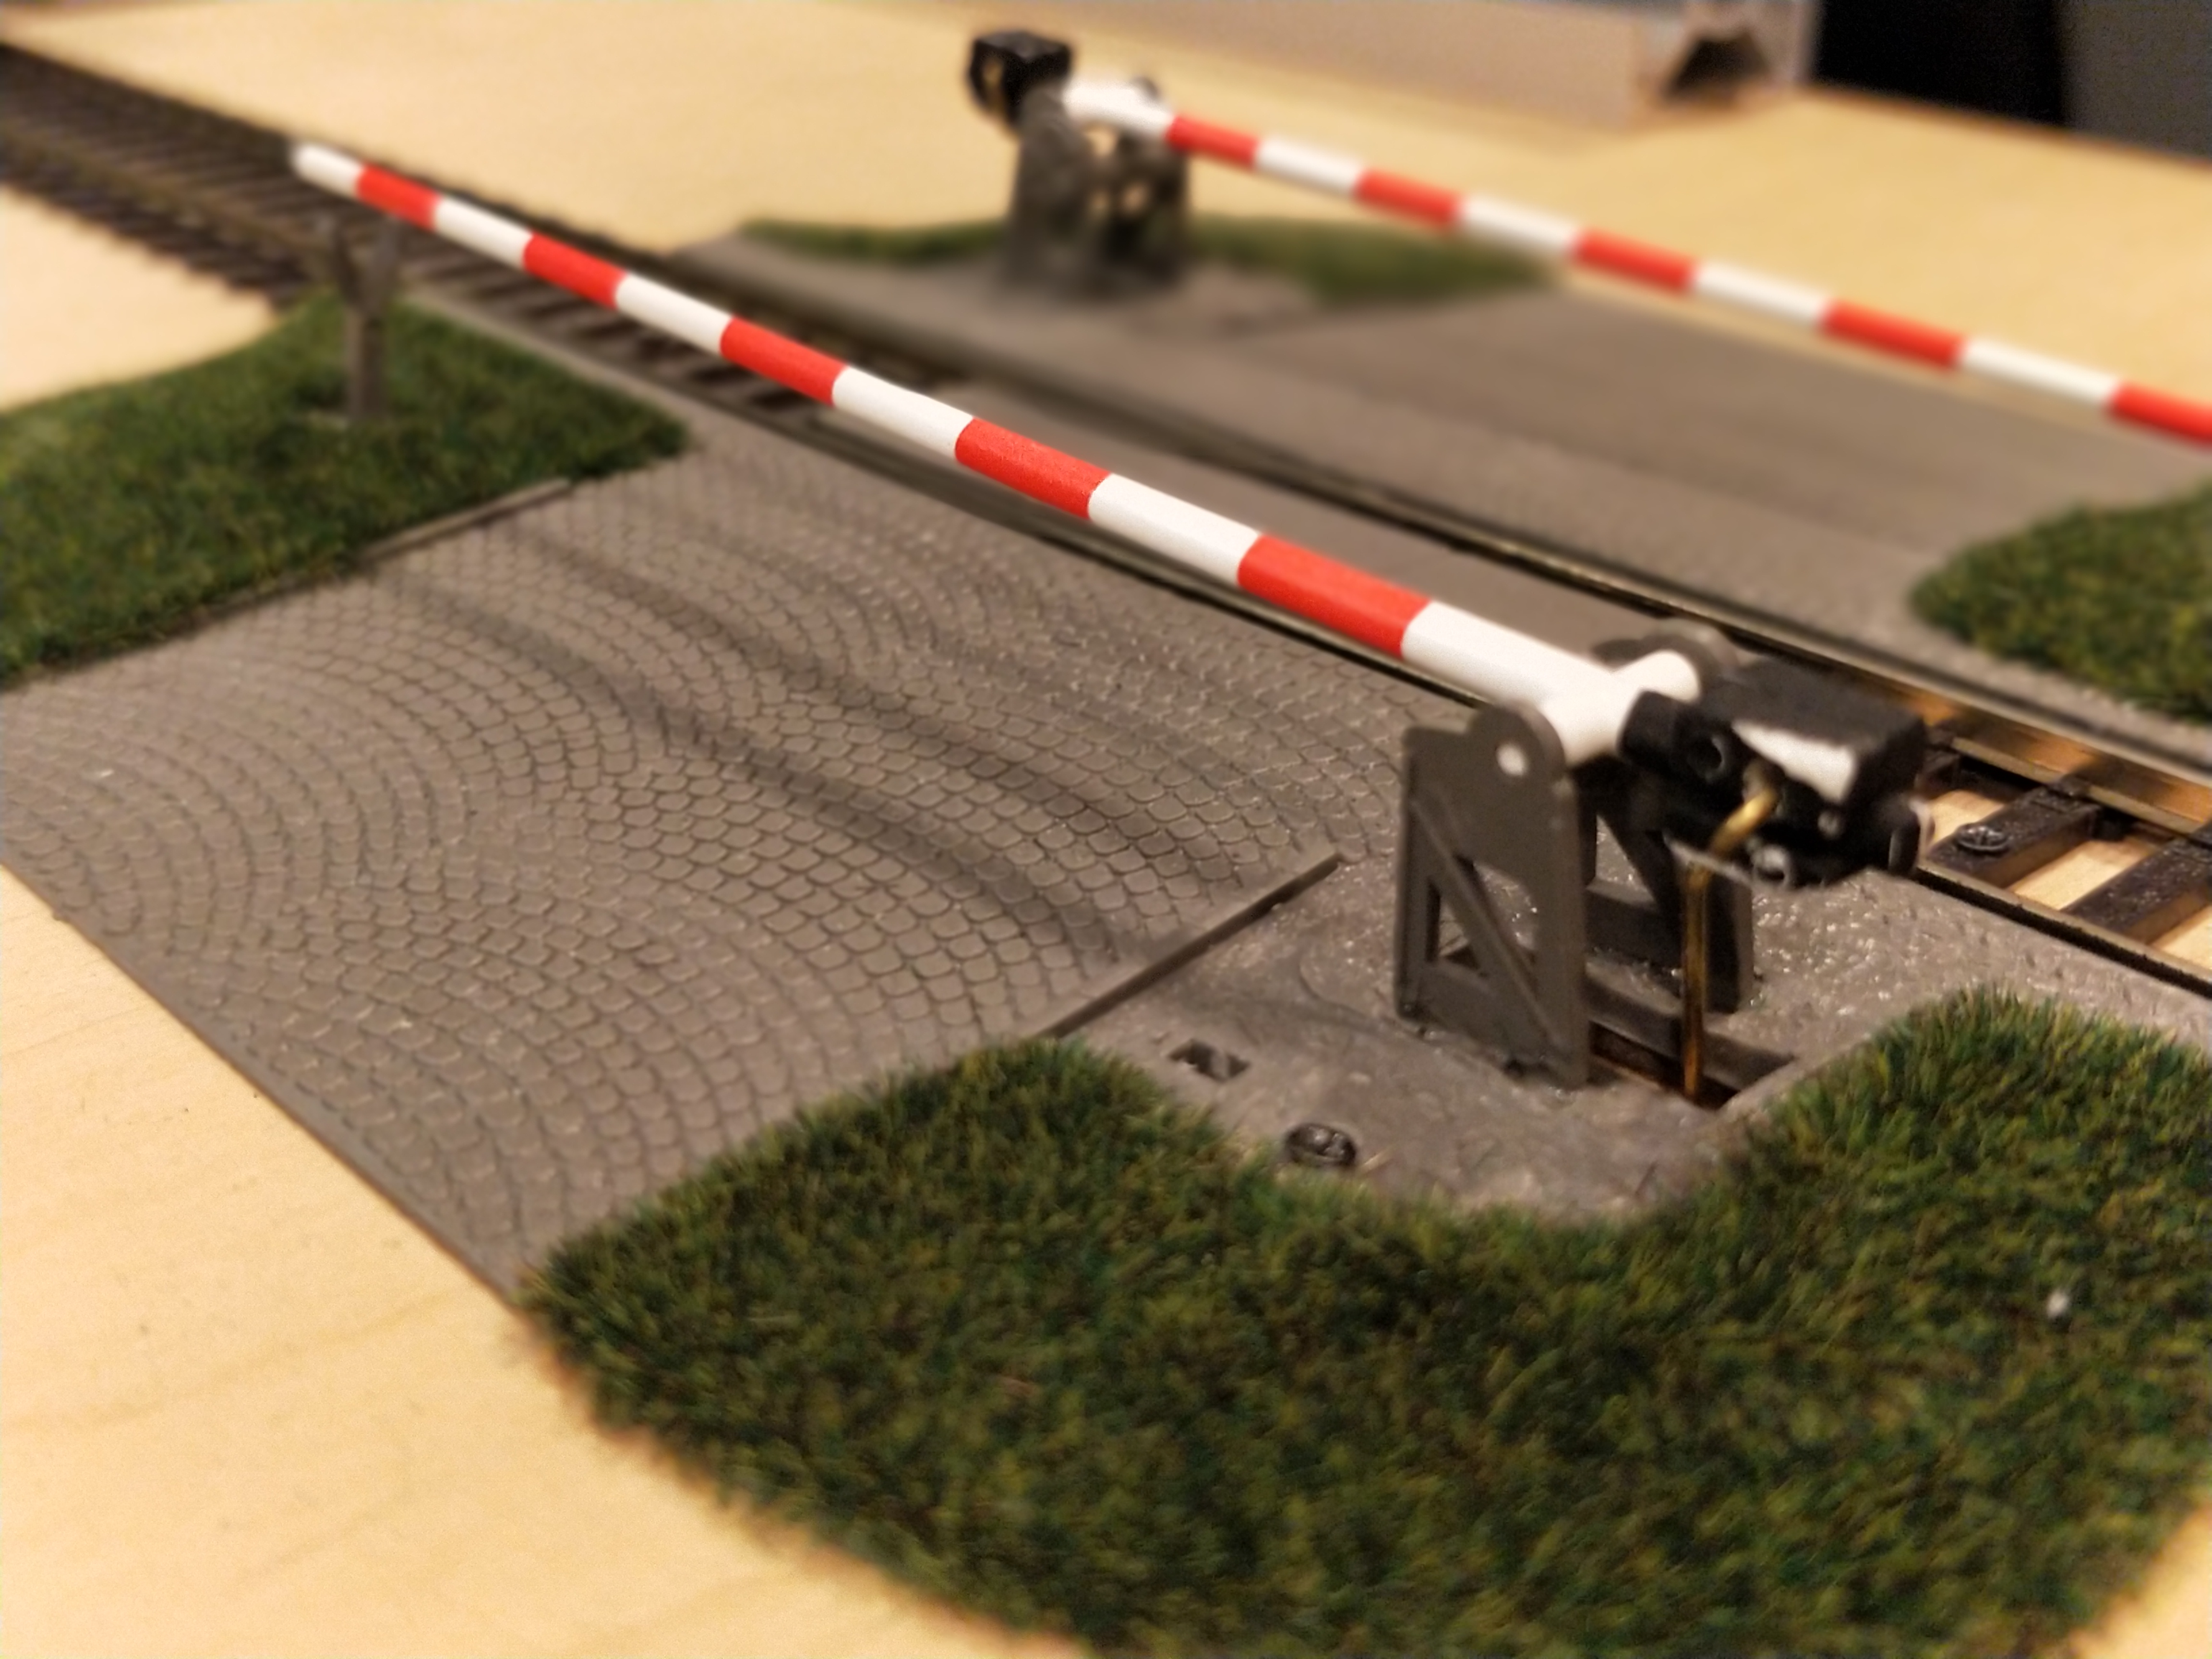
\includegraphics[width=150mm, keepaspectratio]{figures/modes3/barrier.jpg}
%	\caption{Barrier and passageway}
%	\label{fig:barrier}
%\end{figure}
%
%
%\begin{figure}[!h]
%	\centering
%	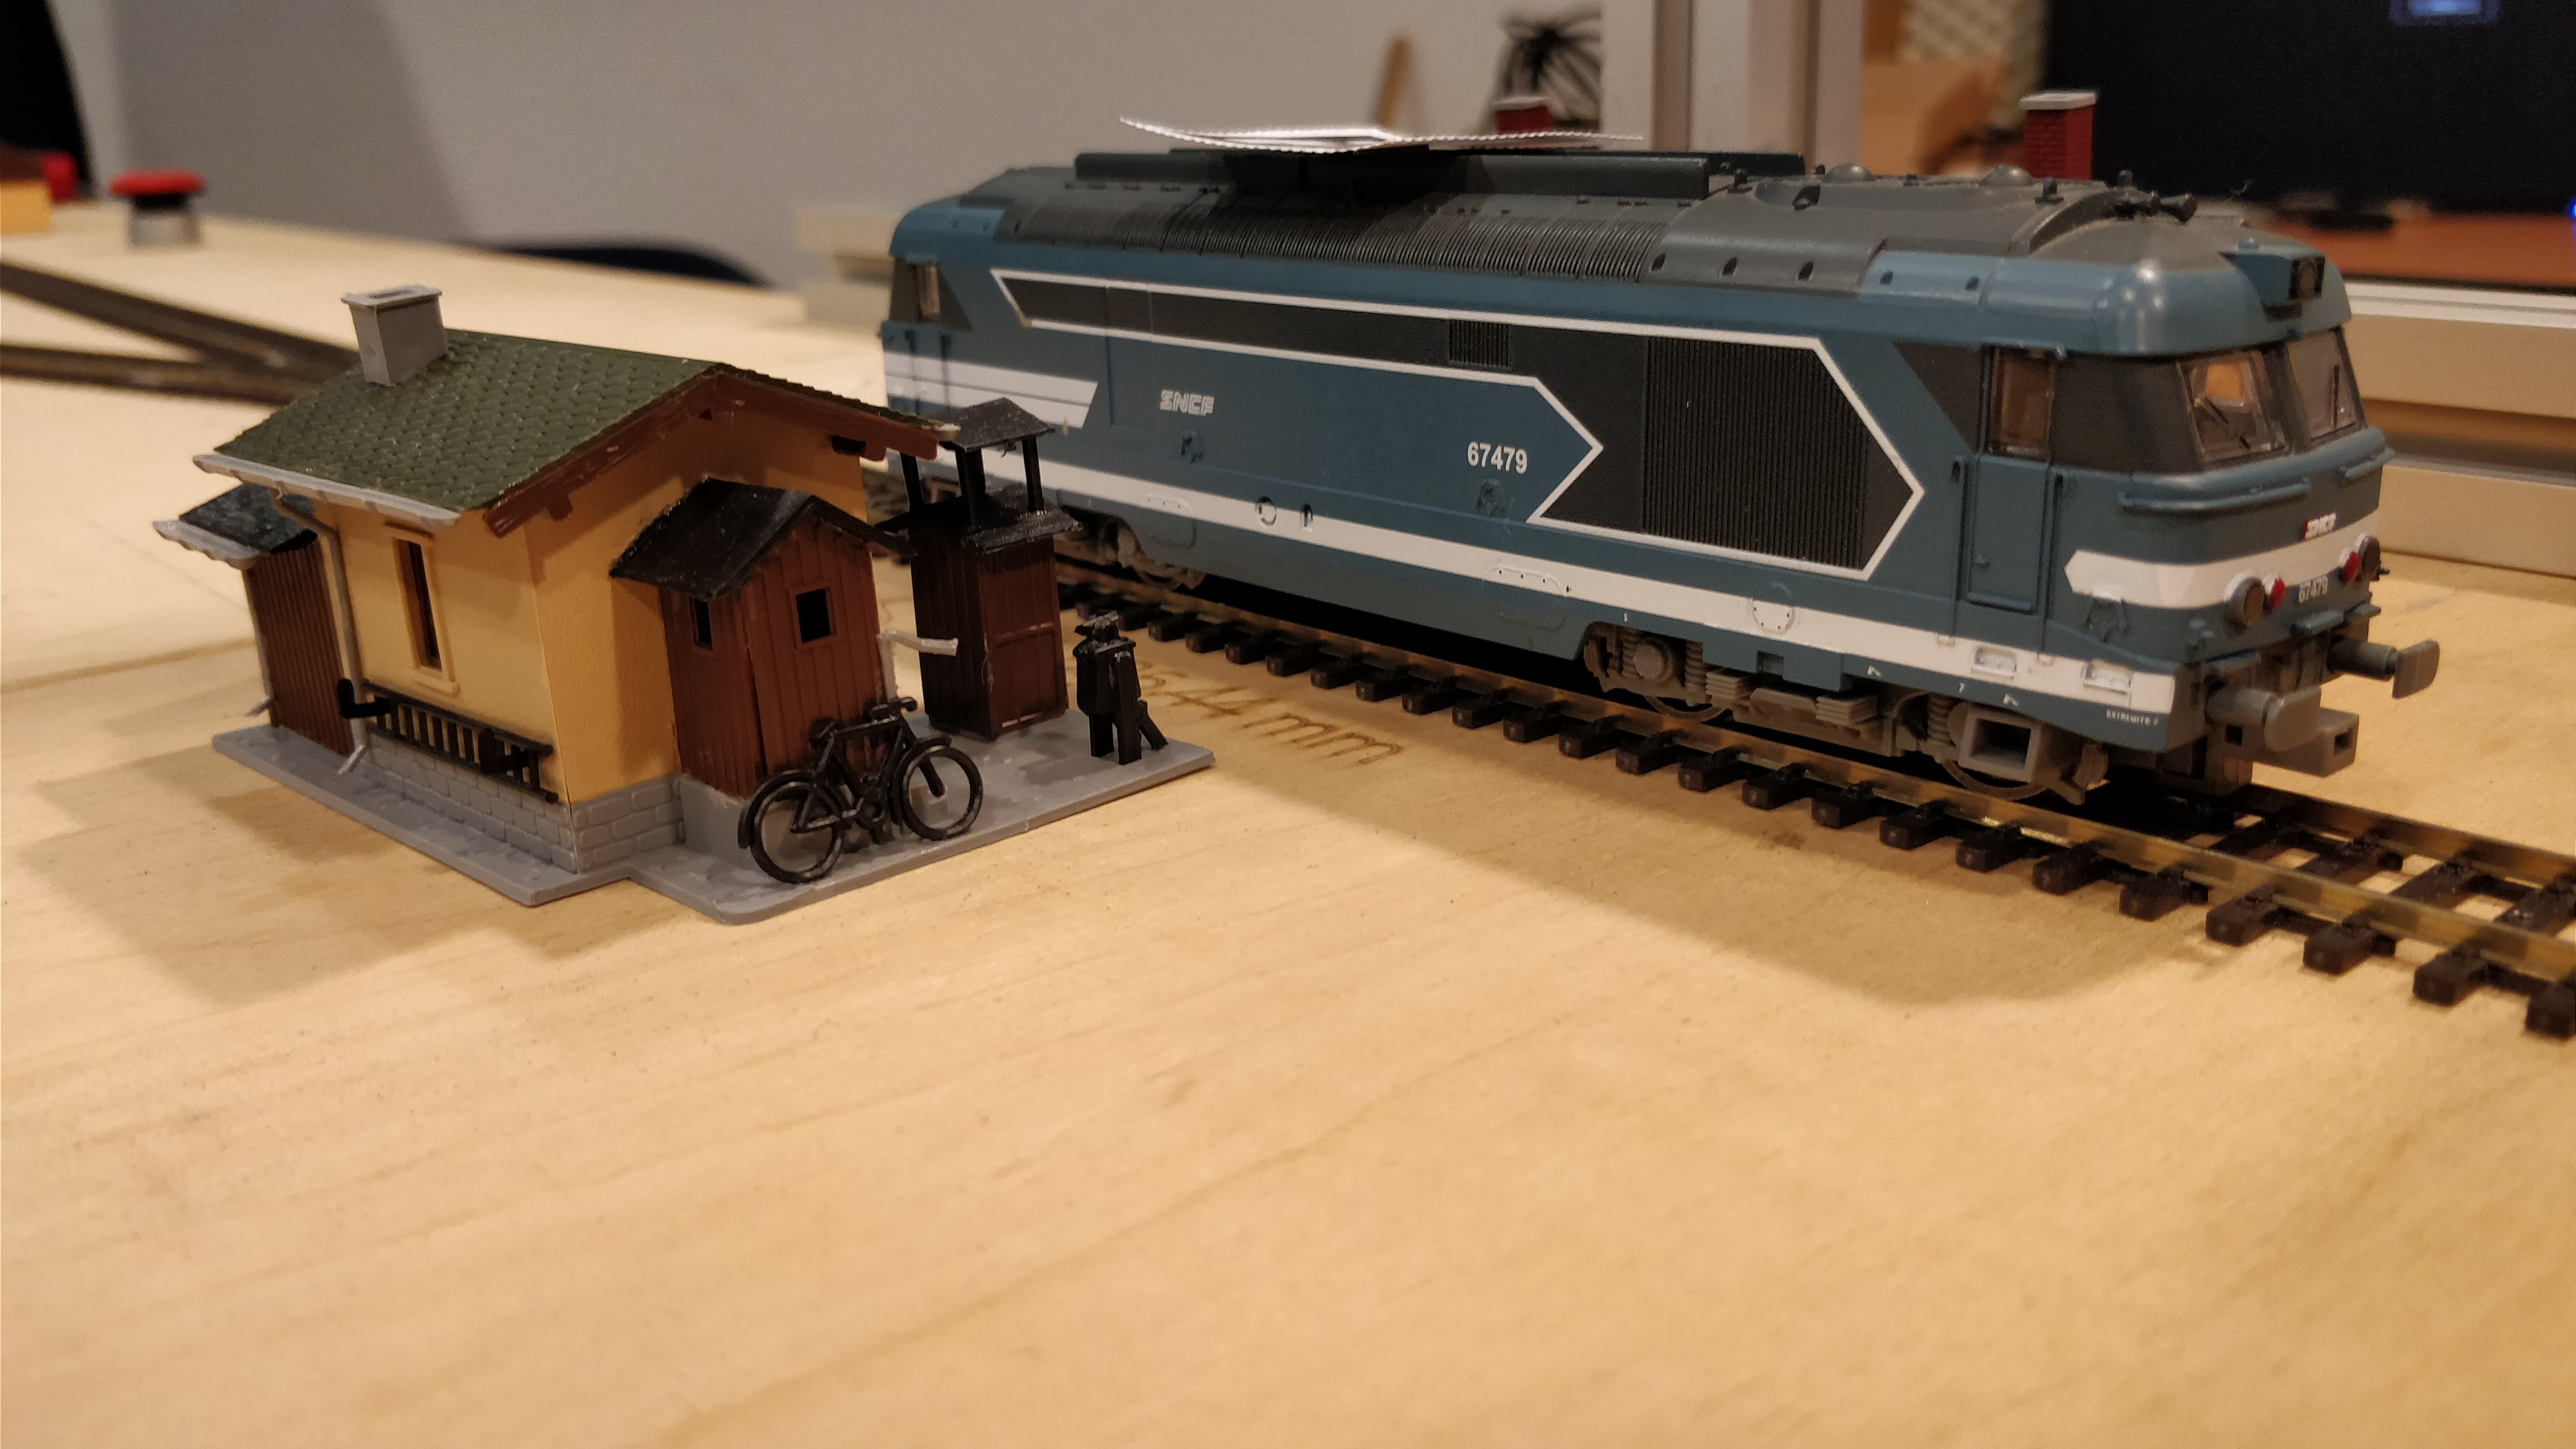
\includegraphics[width=150mm]{figures/modes3/train.jpg}
%	\caption{Train}
%	\label{fig:train}
%\end{figure}
%
\begin{figure}[H]
	\centering
	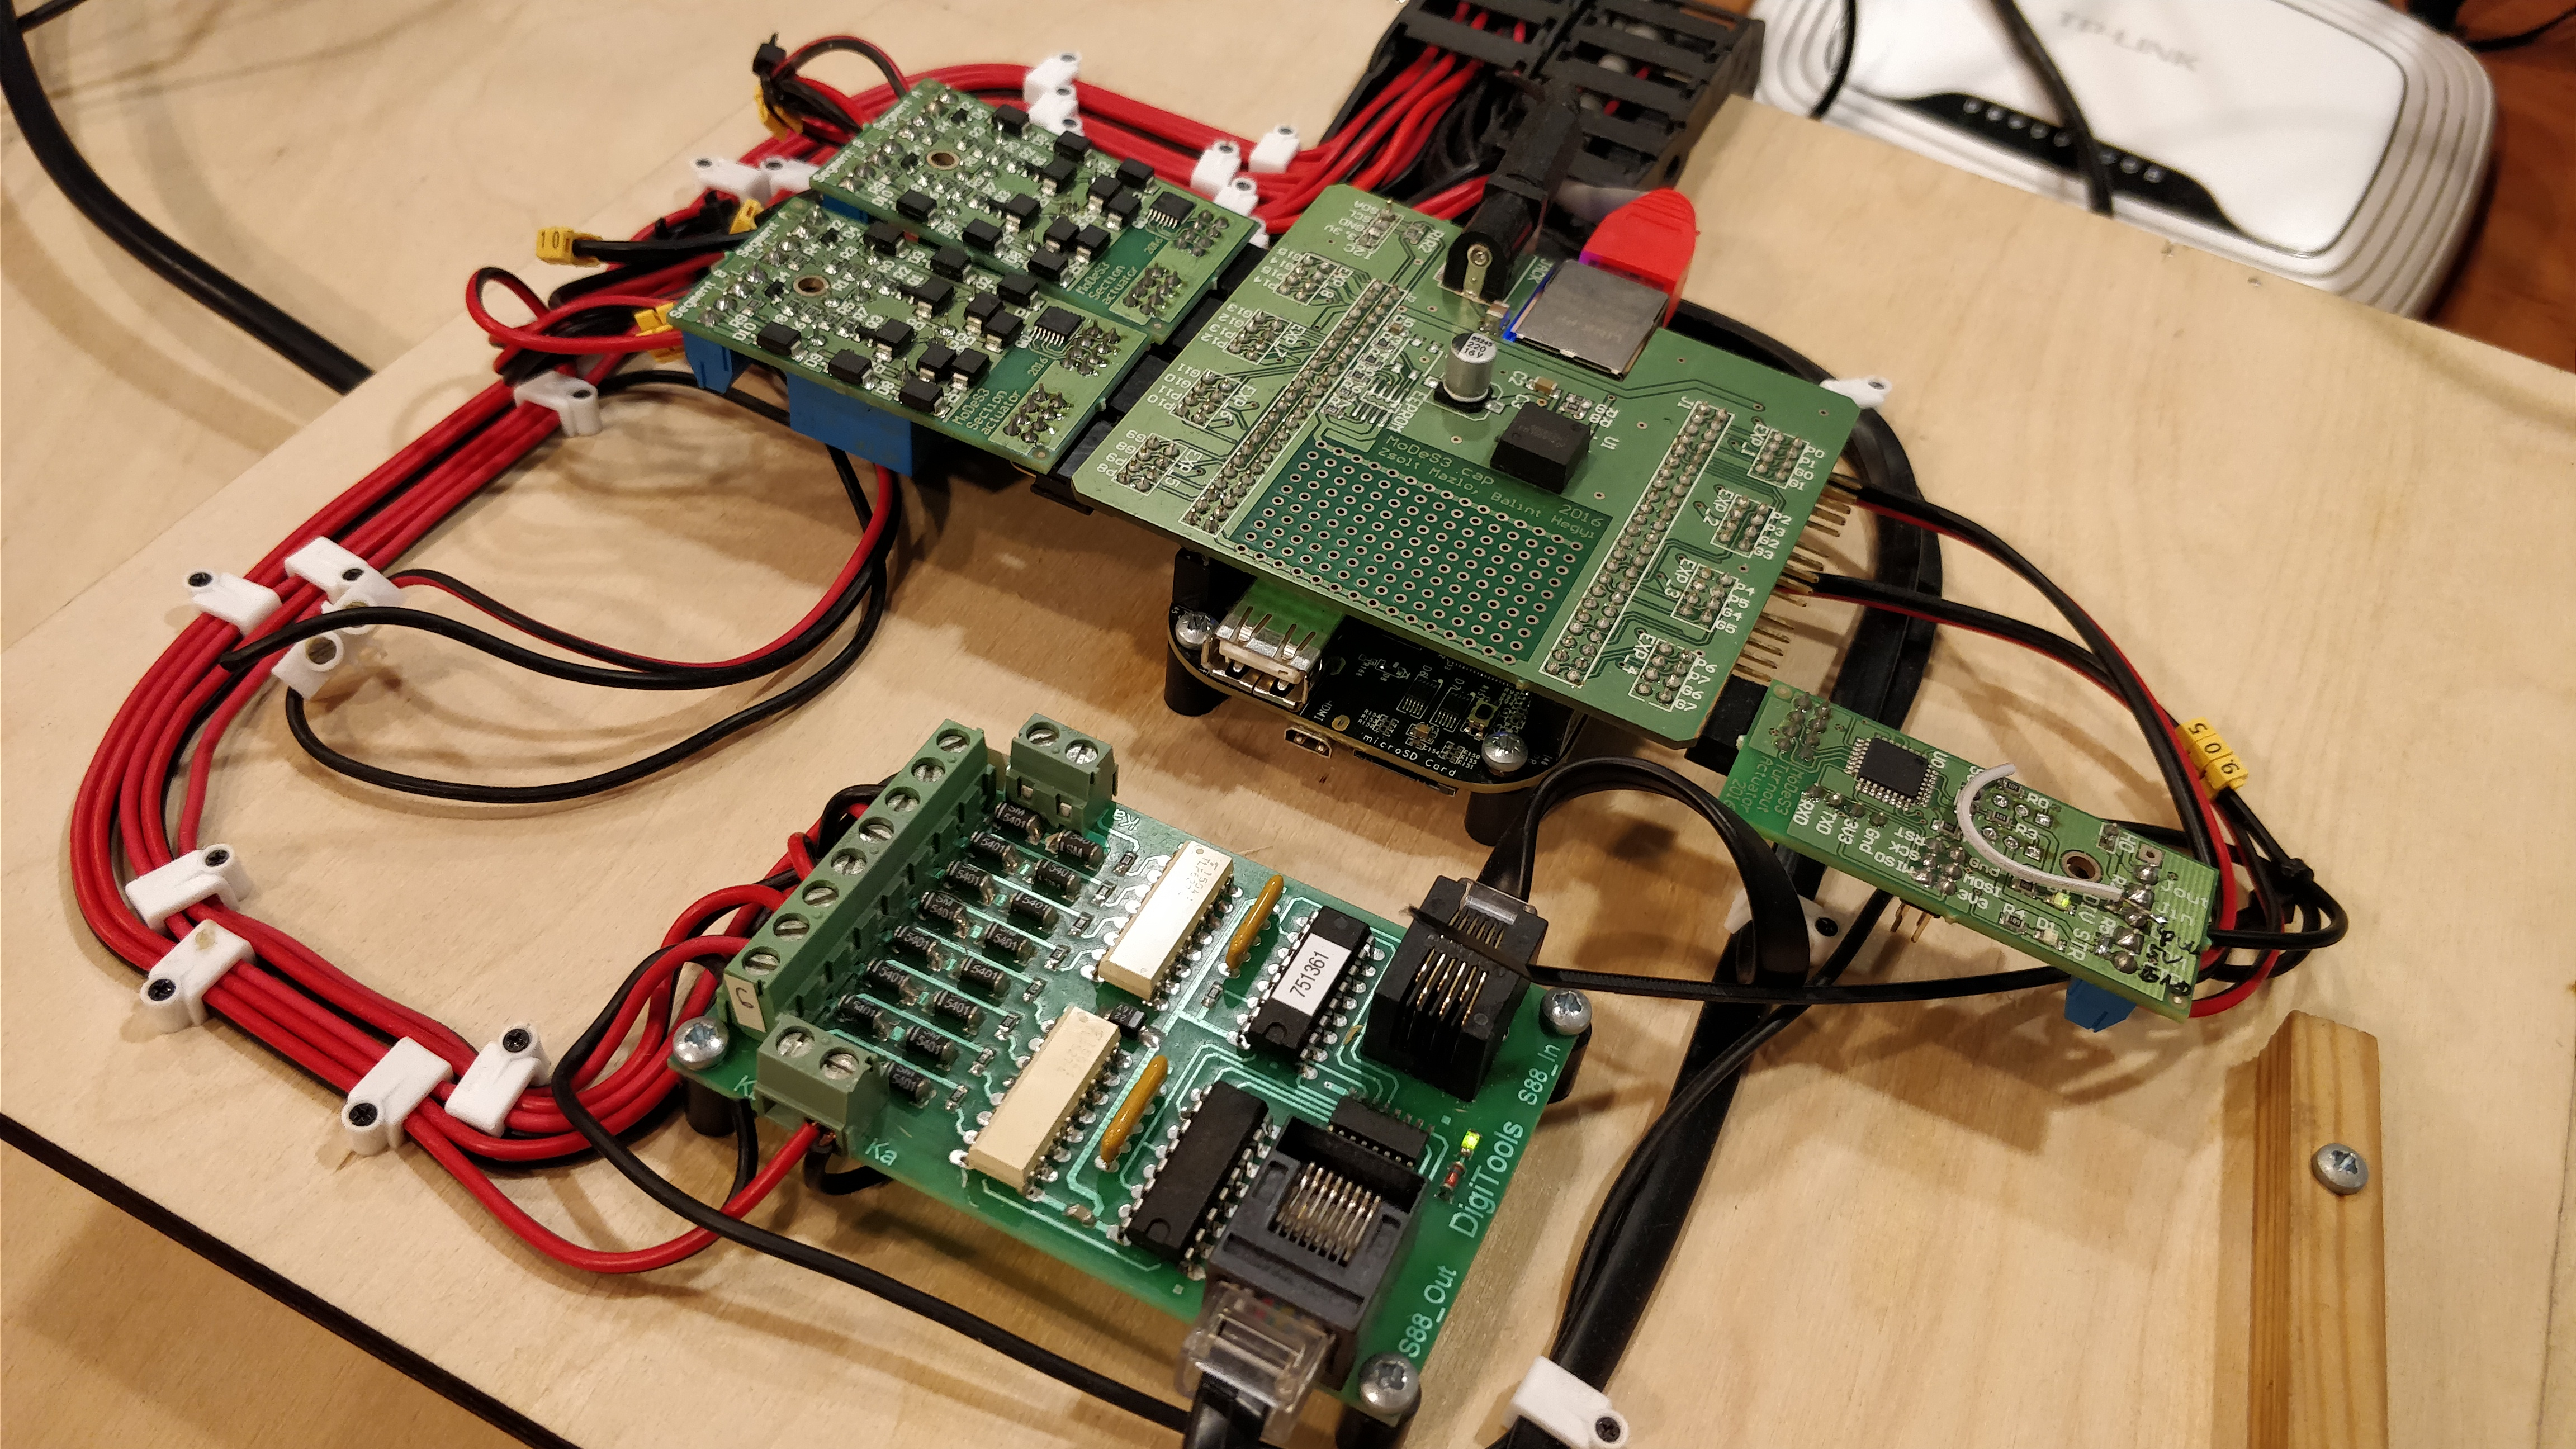
\includegraphics[width=150mm]{figures/modes3/segmentControlling.jpg}
	\caption{Cape, segment and turnout actuator attached to BBB and connection to segment sensor}
	\label{fig:BBBinAll}
\end{figure}
%
%\begin{figure}[!h]
%	\centering
%	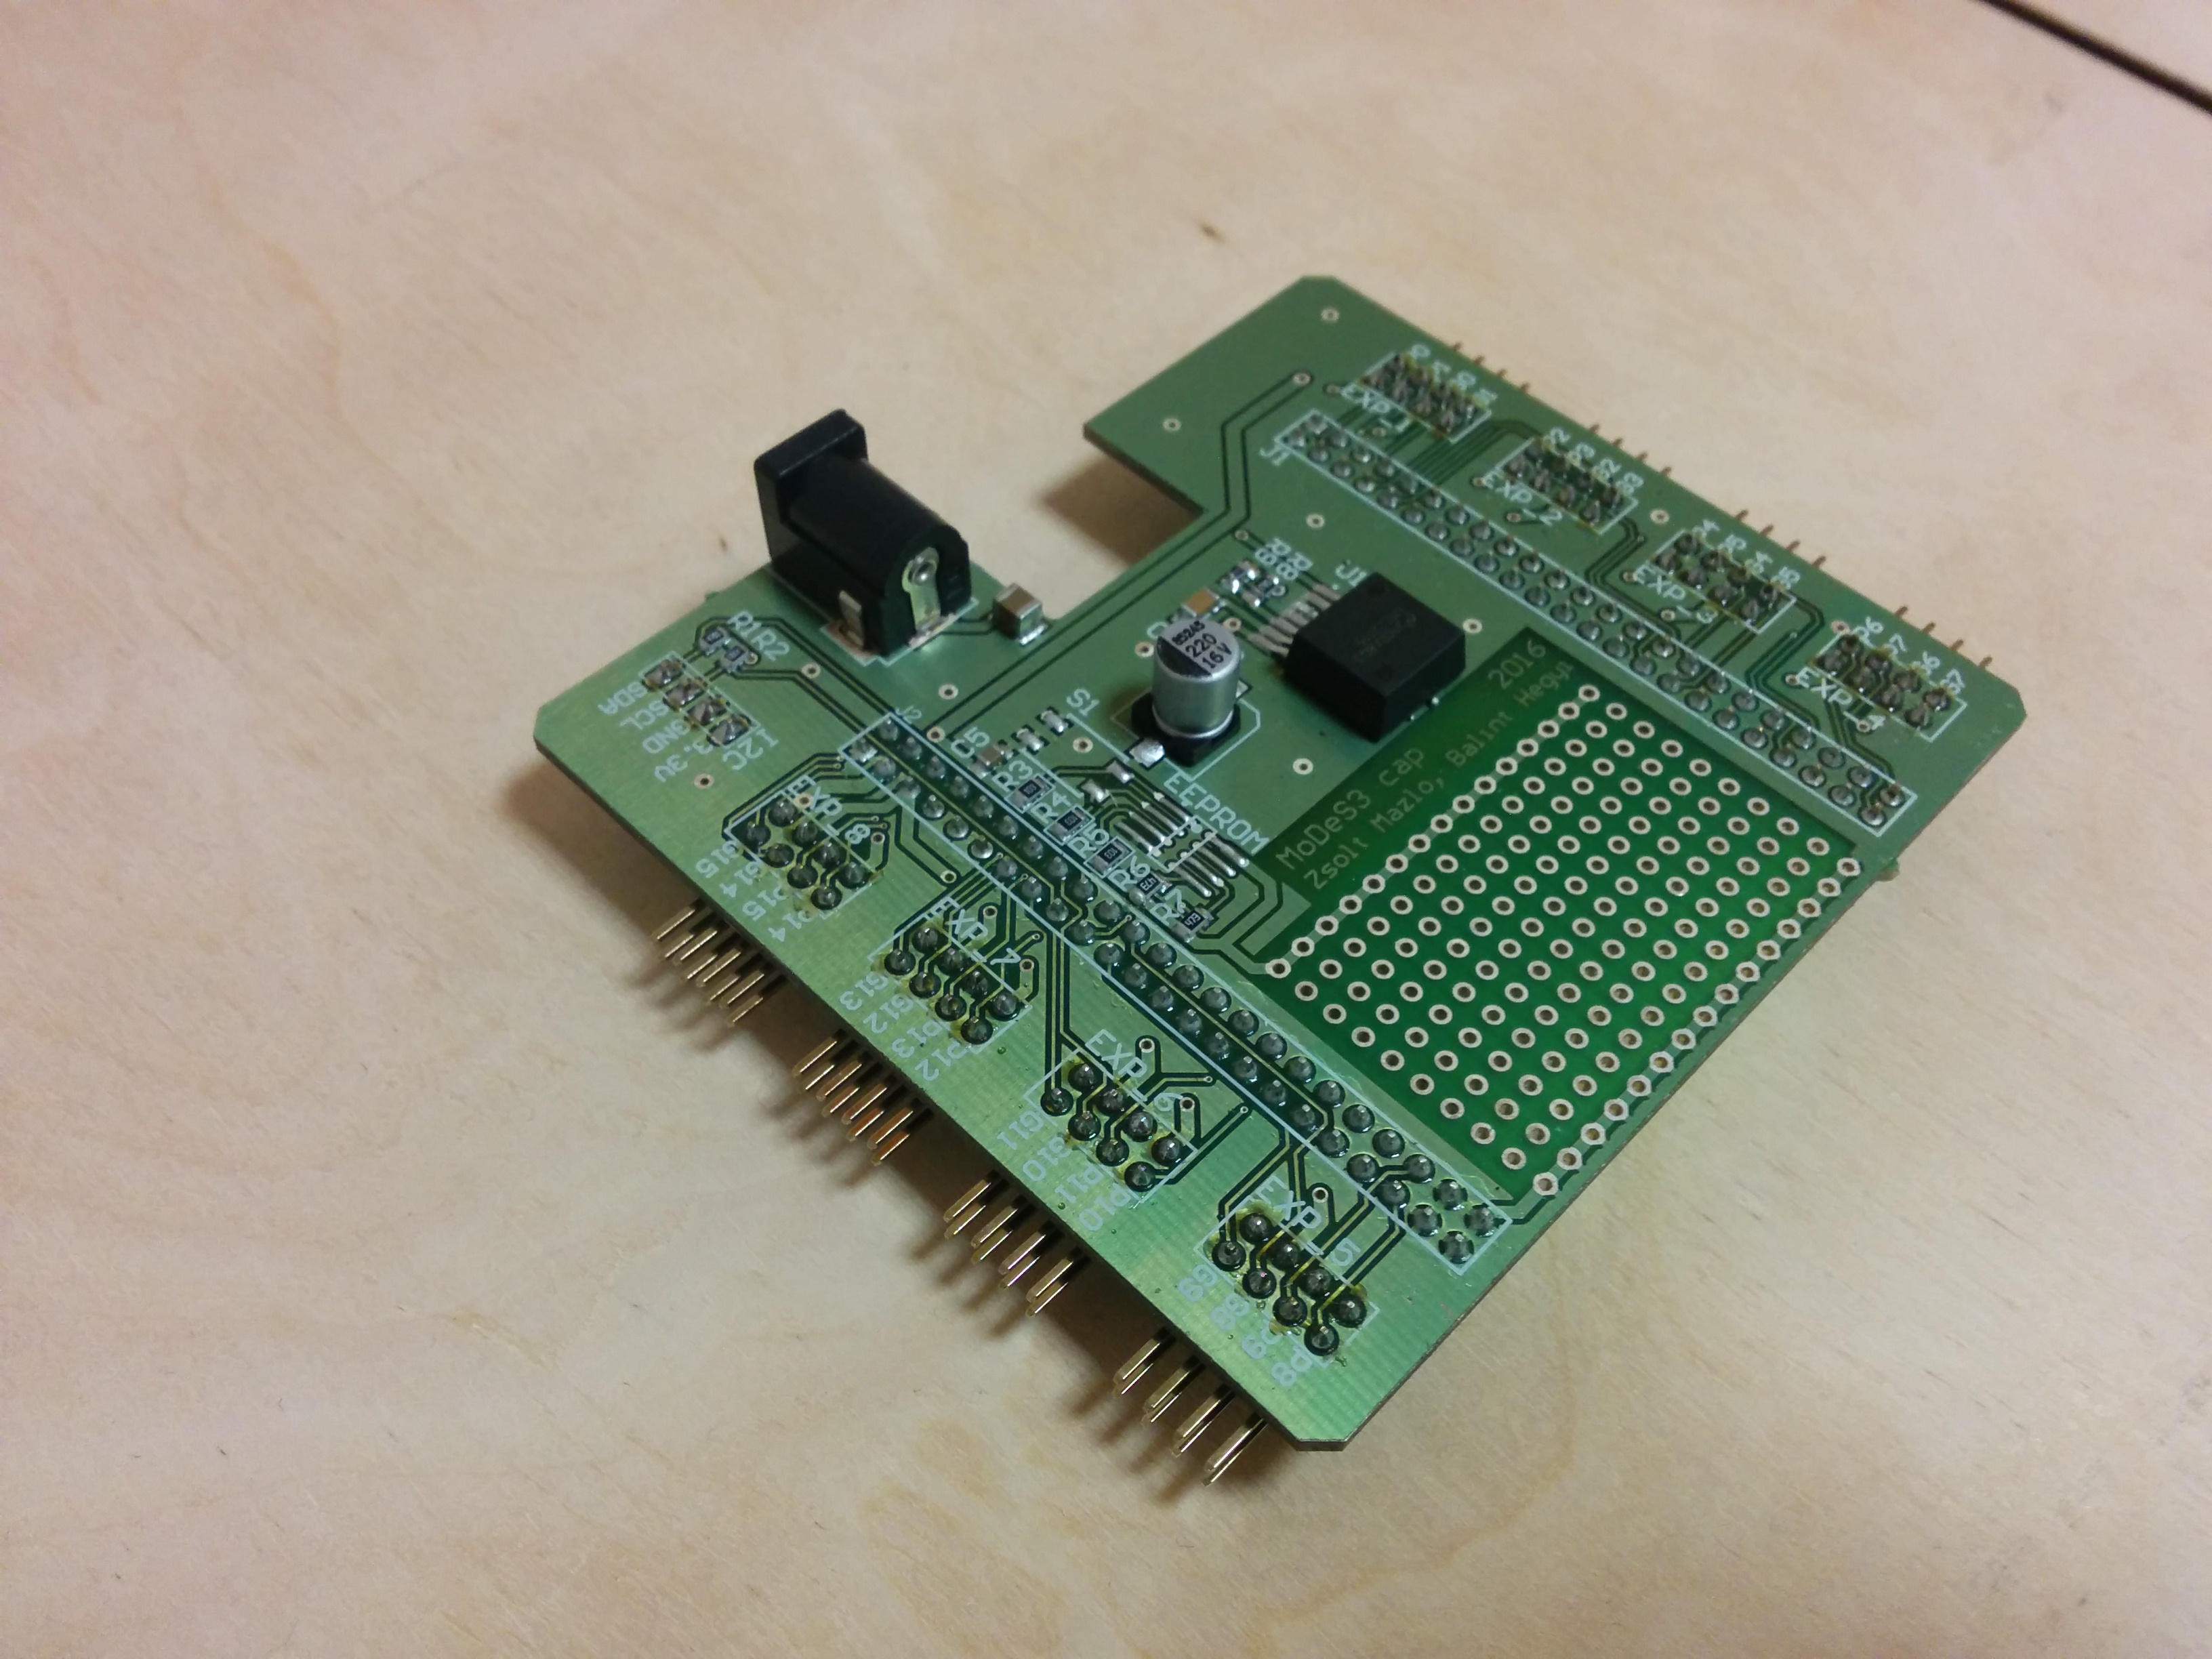
\includegraphics[width=100mm]{figures/modes3/cap1.jpg}
%	\caption{Cape and expander for BeagleBone Black}
%	\label{fig:cape}
%\end{figure}
%
%\begin{figure}[!h]
%	\centering
%	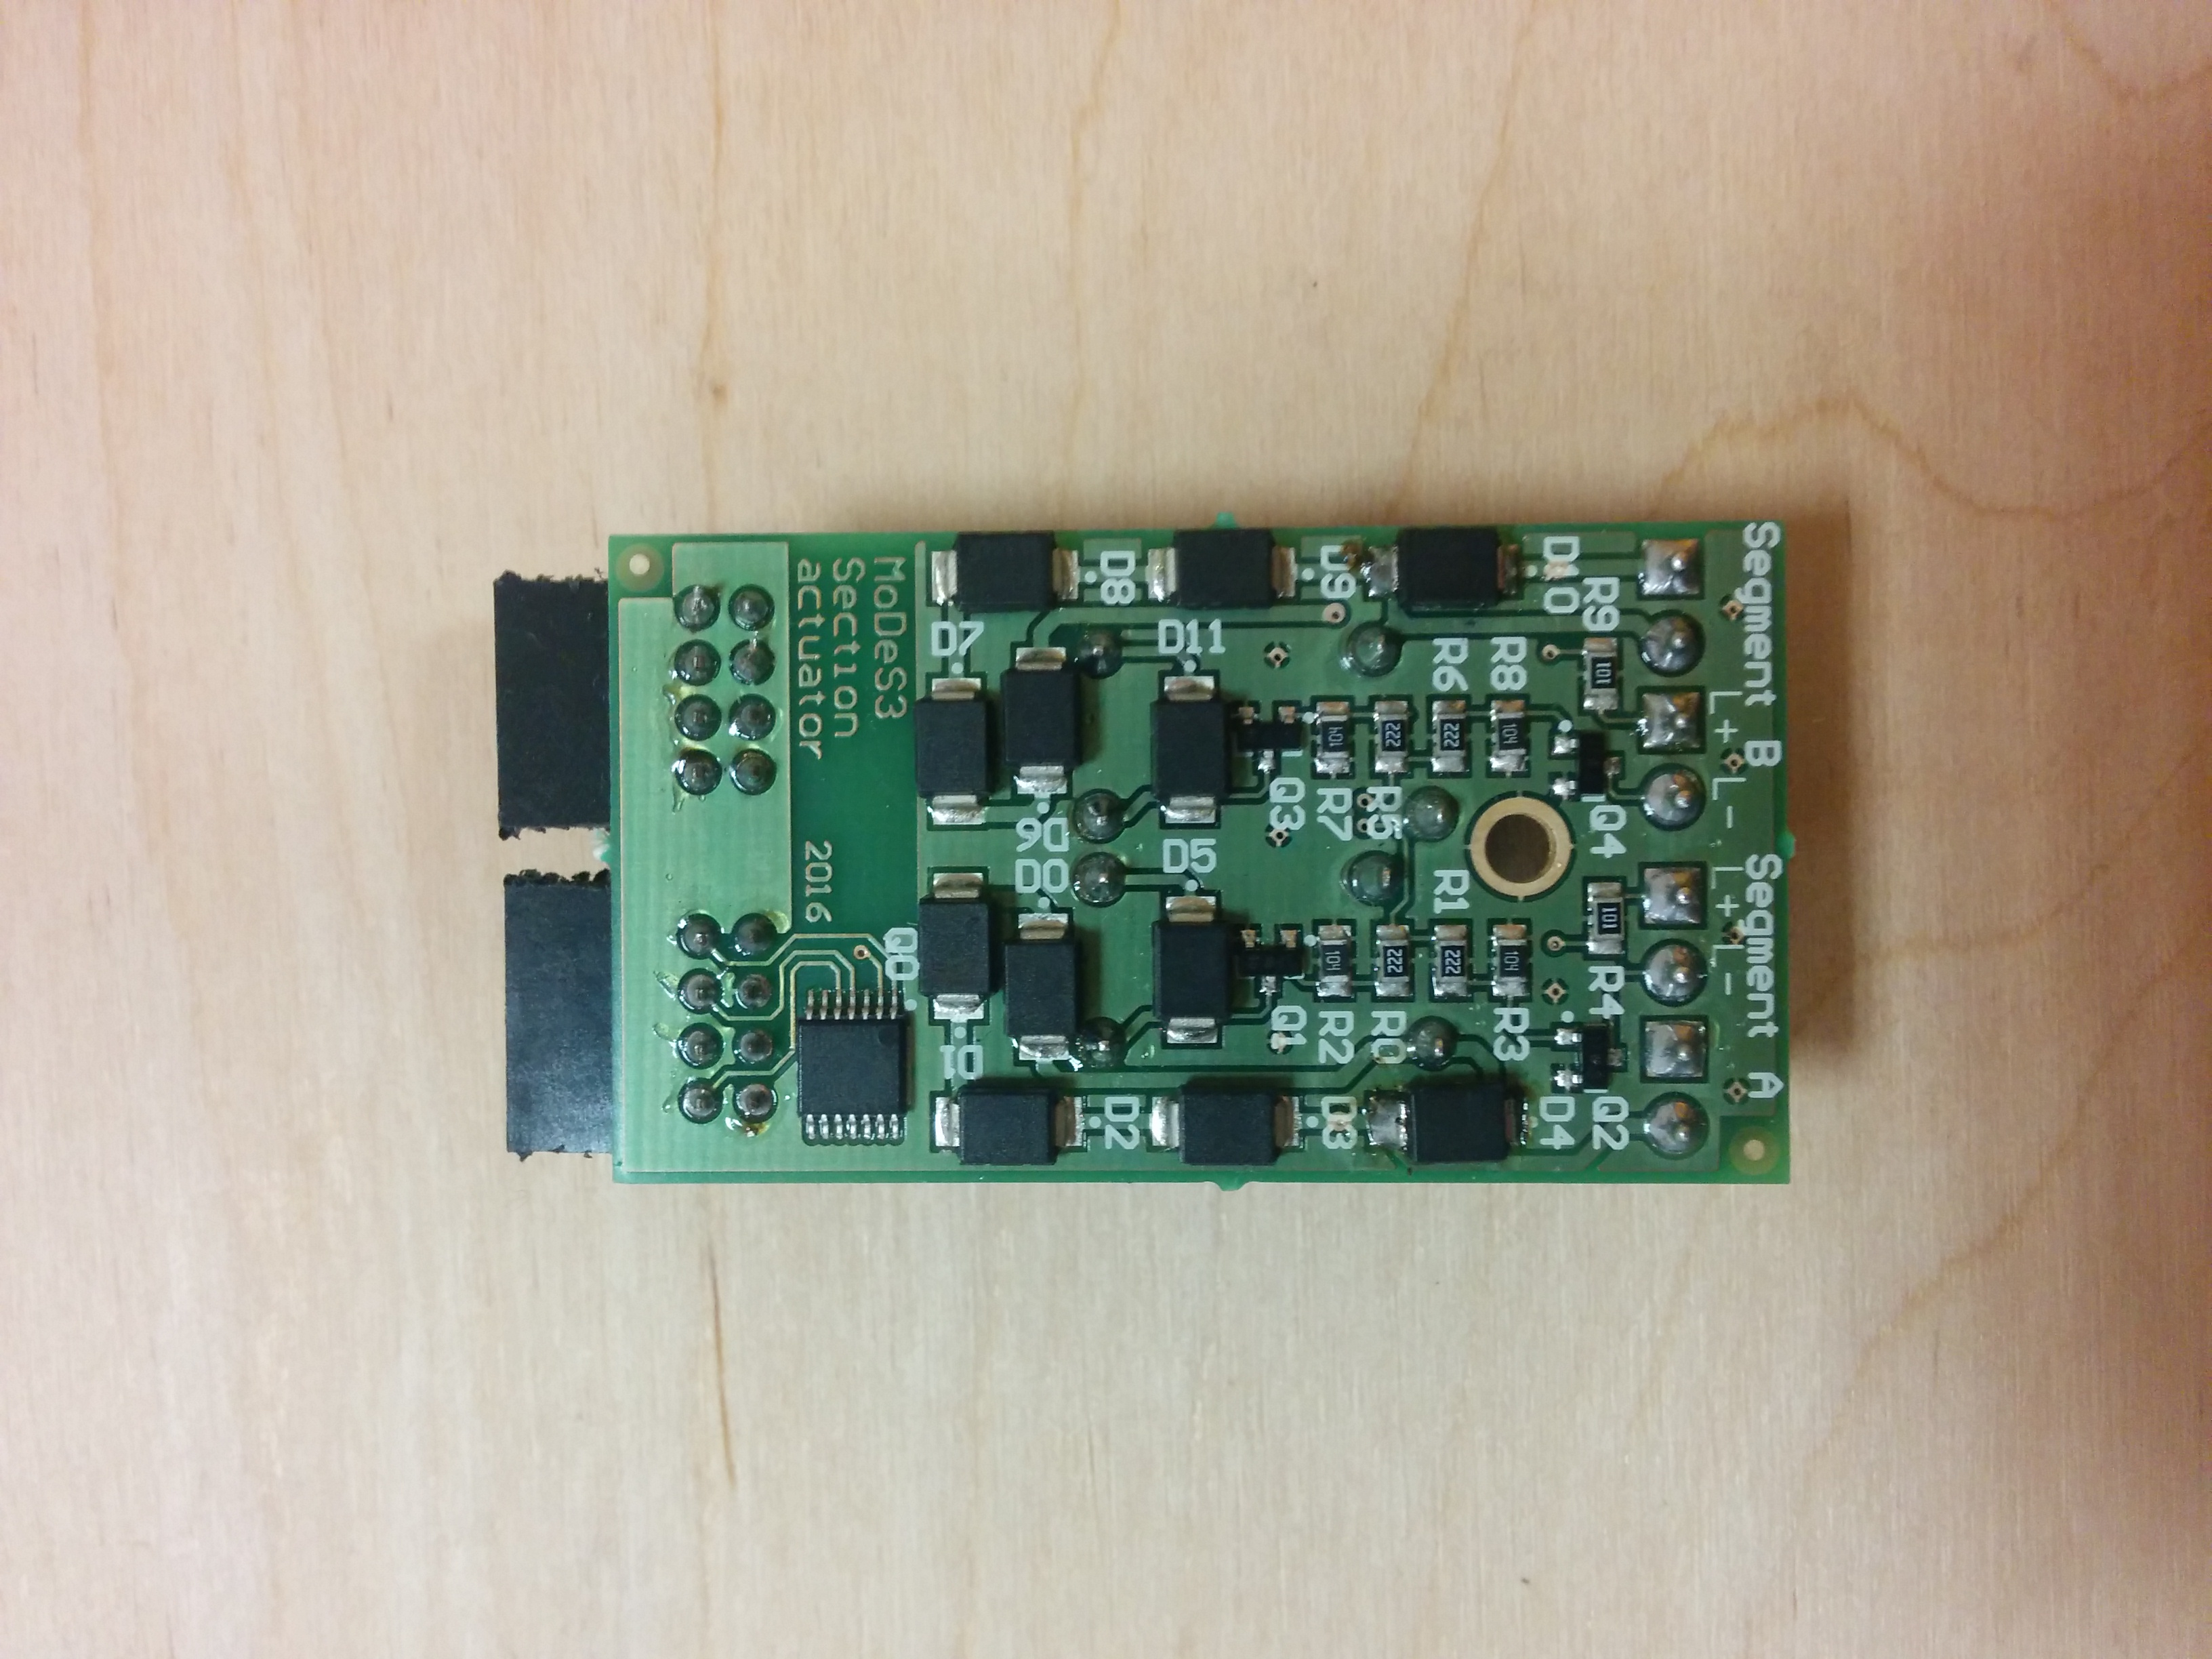
\includegraphics[width=100mm]{figures/modes3/segment-top.jpg}
%	\caption{Segment actuator top view}
%	\label{fig:segmentTop}
%\end{figure}
%
%\begin{figure}[!h]
%	\centering
%	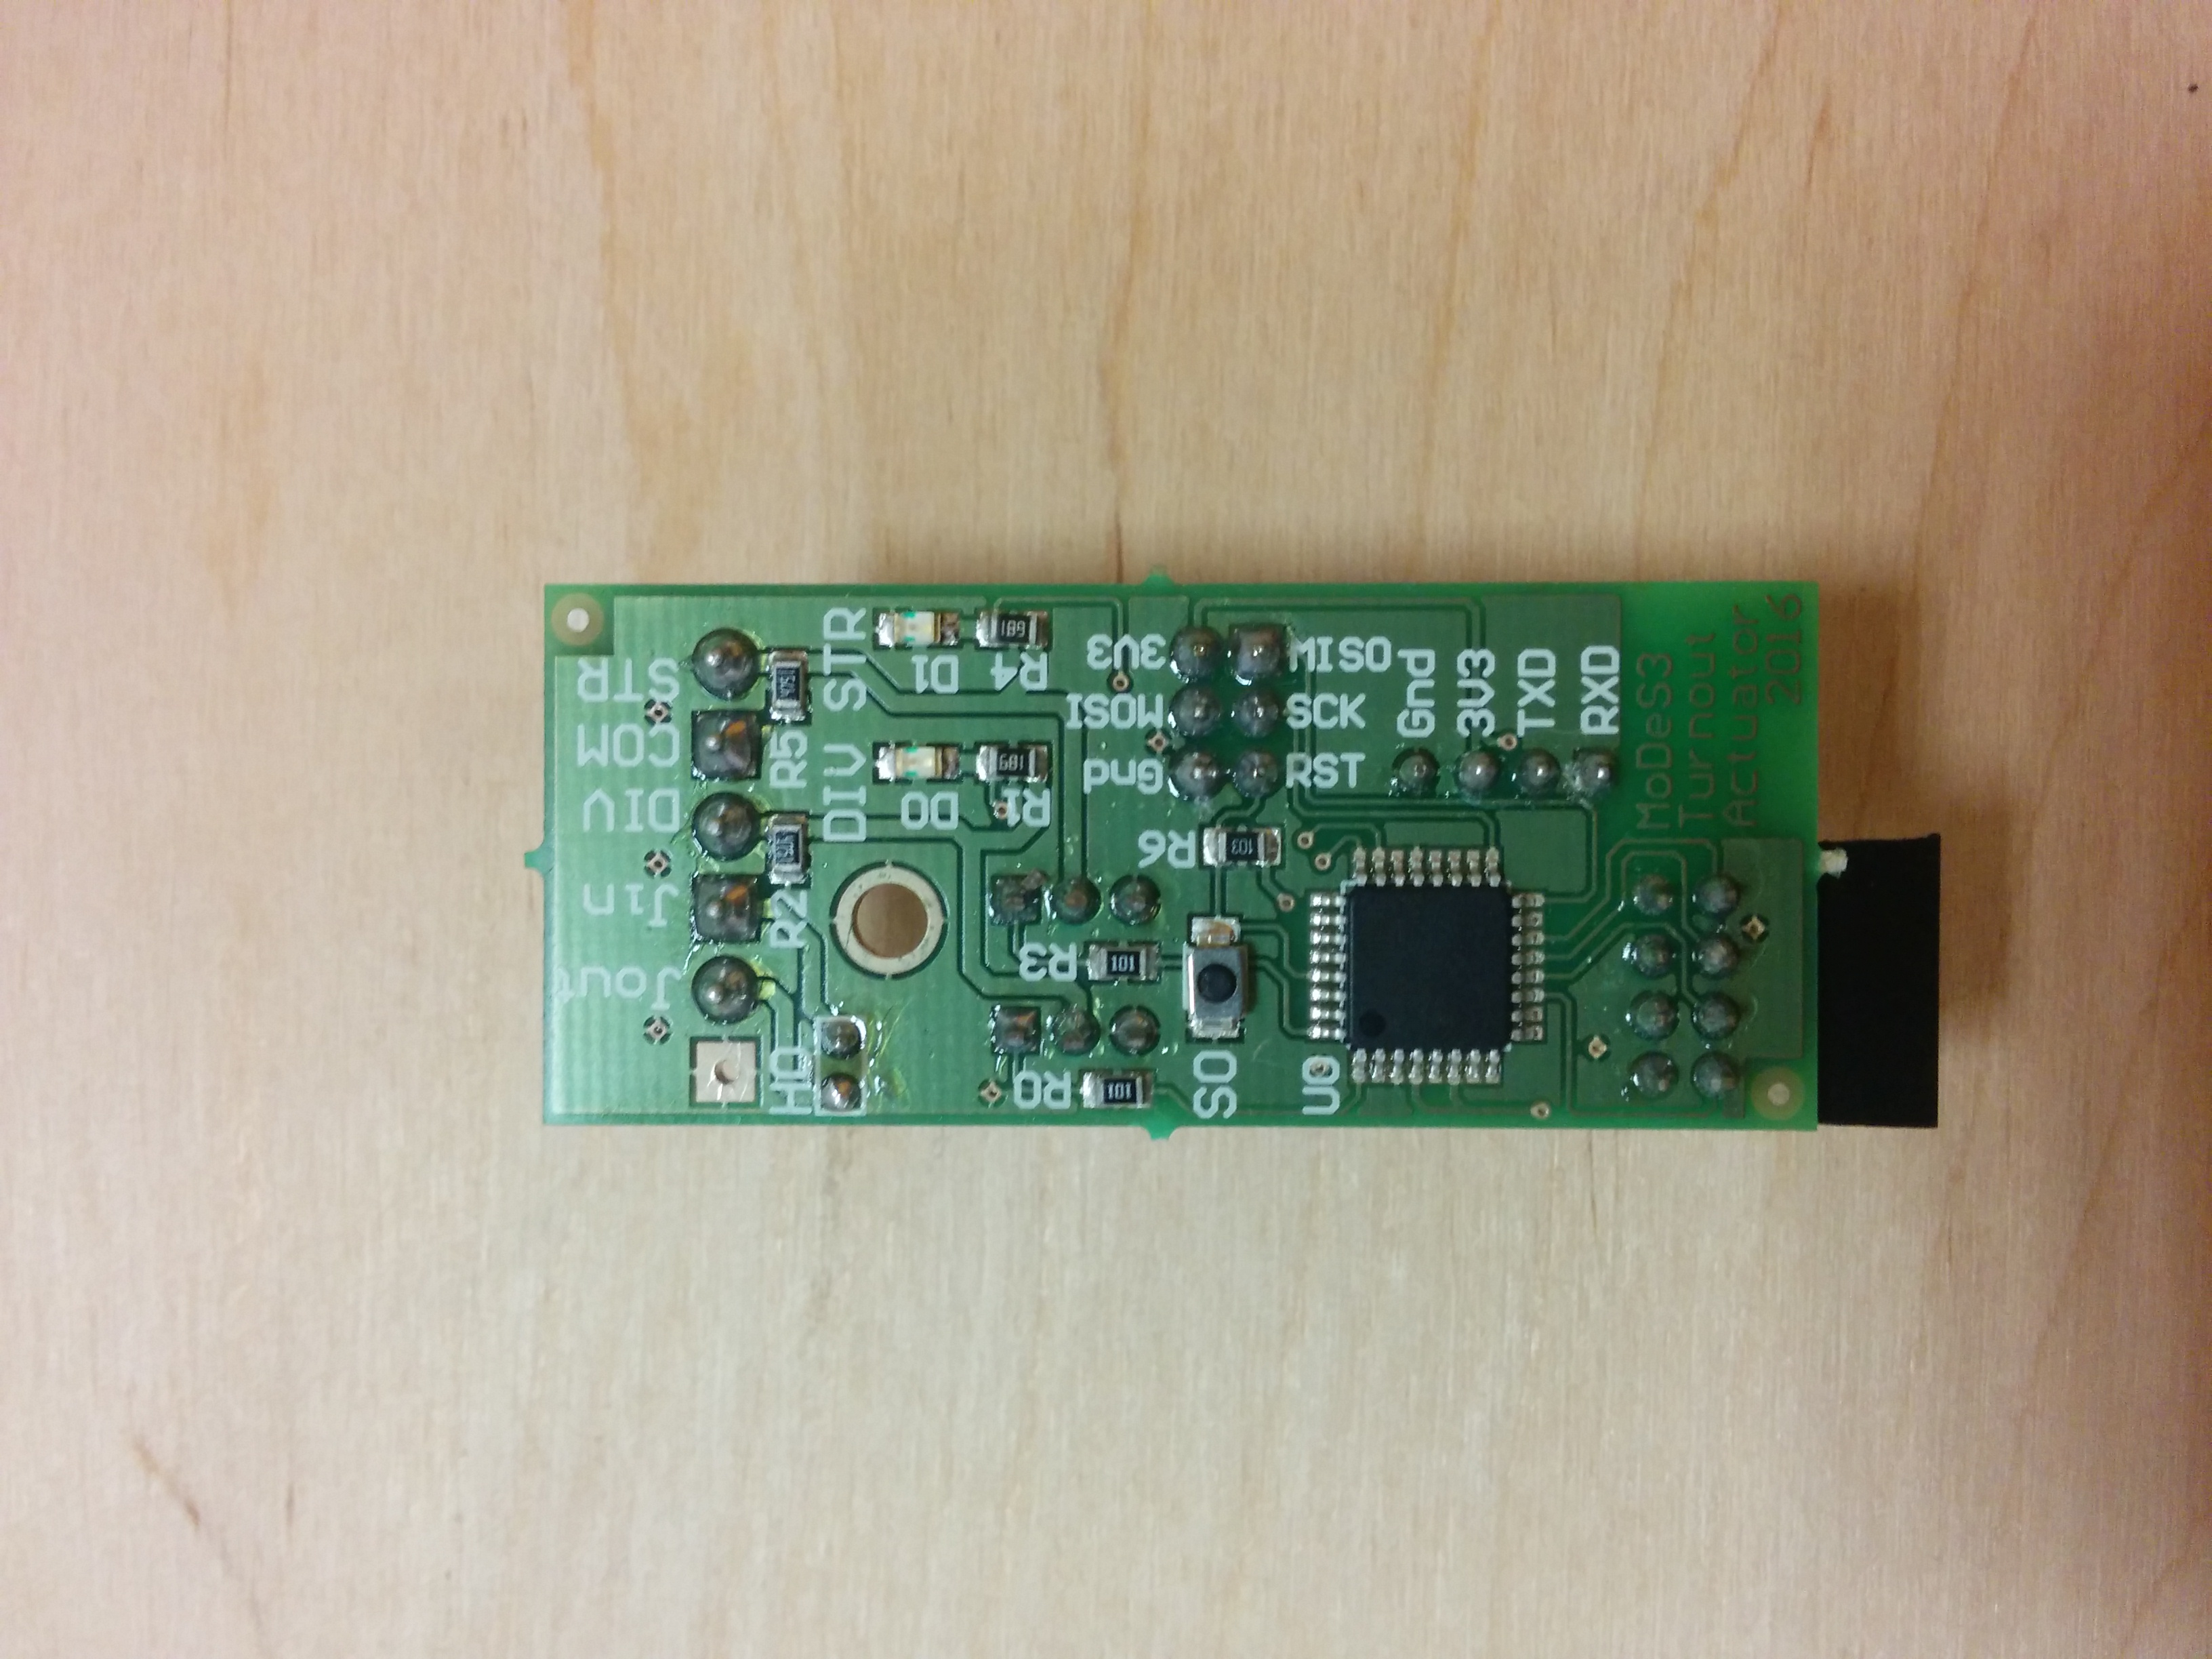
\includegraphics[width=100mm]{figures/modes3/turnout-top.jpg}
%	\caption{Turnout actuator top view}
%	\label{fig:turnoutTop}
%\end{figure}


%----------------------------------------------------------------------------
\section{Test cases for MoDeS$^3$ Unit Test Plan} \label{appendix:UnitTC}
%----------------------------------------------------------------------------

\subsection{GPIO manager}
\begin{table}[H]
	\caption{Test case 1-1}
	\label{table:TCase-FS1-1}
	\begin{center}
		\renewcommand{\arraystretch}{1.8}
		\begin{tabu} 
			to 0.9 \textwidth
			{  X[0.3, l] X[l] }
			\toprule
			Test case ID: 1-1 & Purpose: to test the GPIO initialization in input direction. \newline Priority: am \newline Tracing: FS-1/1.0 \\ \midrule
			Precondition      & The GPIO's necessary files are available.                                                                     \\
			Input             & Initialize the GPIO itself with input direction.                                                              \\
			Expected result   & The "both" string have been written to "edge" configuration file.                                             \\ \bottomrule
		\end{tabu}
	\end{center}
\end{table} 

\begin{table}[H]
	\caption{Test case 1-2}
	\label{table:TCase-FS1-2}
	\begin{center}
		\renewcommand{\arraystretch}{1.8}
		\begin{tabu} 
			to 0.9 \textwidth
			{  X[0.3, l] X[l] }
			\toprule
			Test case ID: 1-2 & Purpose: to test the GPIO pin input change listener while direction is input and the value is "0". \newline Priority: am \newline Tracing: FS-1/1.1 \\ \midrule
			Precondition      & The GPIO's necessary files are available.                                                                                                           \\
			Input             & The value file have been written to "0", considered as LOW.                                                                                         \\
			Expected result   & GPIO noticed the change and read the "value" configuration file content as LOW level.                                                               \\ \bottomrule
		\end{tabu}
	\end{center}
\end{table} 

\begin{table}[H]
	\caption{Test case 1-3}
	\label{table:TCase-FS1-3}
	\begin{center}
		\renewcommand{\arraystretch}{1.8}
		\begin{tabu} 
			to 0.9 \textwidth
			{  X[0.3, l] X[l] }
			\toprule
			Test case ID: 1-3 & Purpose: to test the GPIO pin change listener while direction is input and the value is "1". \newline Priority: am \newline Tracing: FS-1/1.2 \\ \midrule
			Precondition      & The GPIO's necessary files are available.                                                                                                     \\
			Input             & The value file have been written to "1" considered as HIGH.                                                                                   \\
			Expected result   & GPIO noticed the change and read the "value" configuration file content as HIGH level.                                                        \\ \bottomrule
		\end{tabu}
	\end{center}
\end{table} 

\begin{table}[H]
	\caption{Test case 1-4}
	\label{table:TCase-FS1-4}
	\begin{center}
		\renewcommand{\arraystretch}{1.8}
		\begin{tabu} 
			to 0.9 \textwidth
			{  X[0.3, l] X[l] }
			\toprule
			Test case ID: 1-4 & Purpose: to test the GPIO initialization in output direction. \newline Priority: am \newline Tracing: FS-1/2.0 \\ \midrule
			Precondition      & The GPIO's necessary files are available.                                                                      \\
			Input             & Initialize the GPIO itself with output direction.                                                              \\
			Expected result   & The "0" string have been written to "value" configuration file.                                                \\ \bottomrule
		\end{tabu}
	\end{center}
\end{table} 

\begin{table}[H]
	\caption{Test case 1-5}
	\label{table:TCase-FS1-5}
	\begin{center}
		\renewcommand{\arraystretch}{1.8}
		\begin{tabu} 
			to 0.9 \textwidth
			{  X[0.3, l] X[l] }
			\toprule
			Test case ID: 1-5 & Purpose: to test the GPIO pin's level setting to LOW. \newline Priority: am \newline Tracing: FS-1/2.1 \\ \midrule
			Precondition      & The GPIO's necessary files are available.                                                              \\
			Input             & Set the GPIO's level to LOW.                                                                           \\
			Expected result   & The "value" file has been modified with value "0"                                                      \\ \bottomrule
		\end{tabu}
	\end{center}
\end{table} 

\begin{table}[H]
	\caption{Test case 1-6}
	\label{table:TCase-FS1-6}
	\begin{center}
		\renewcommand{\arraystretch}{1.8}
		\begin{tabu} 
			to 0.9 \textwidth
			{  X[0.3, l] X[l] }
			\toprule
			Test case ID: 1-6 & Purpose: to test the GPIO pin's level setting to HIGH.  \newline Priority: am \newline Tracing: FS-1/2.2 \\ \midrule
			Precondition      & The GPIO's necessary files are available.                                                                \\
			Input             & Set the GPIO's level to HIGH.                                                                            \\
			Expected result   & The "value" file has been modified with value "1"                                                        \\ \bottomrule
		\end{tabu}
	\end{center}
\end{table} 

\subsection{Occupancy detection}

\begin{table}[H]
	\caption{Test case 2-1}
	\label{table:TCase-FS2-1}
	\begin{center}
		\renewcommand{\arraystretch}{1.8}
		\begin{tabu} 
			to 0.9 \textwidth
			{  X[0.3, l] X[l] }
			\toprule
			Test case ID: 2-1 & Purpose: to test the detection of segment occupancy (the train power consumption) through section occupancy query, when the specific segment is free\newline Priority: above middle \newline Tracing: (FS-2/1.0) \\ \midrule
			Precondition      & S88 serial port connection and available Arduino hardware element                                                                                                                                                \\
			Input             & Unclosed circuit between the specific segment's hardware elements elements                                                                                                                                       \\
			Expected result   & Occupancy components have queried free occupancy state                                                                                                                                                           \\ \bottomrule
		\end{tabu}
	\end{center}
\end{table} 

\begin{table}[H]
	\caption{Test case 2-2}
	\label{table:TCase-FS2-2}
	\begin{center}
		\renewcommand{\arraystretch}{1.8}
		\begin{tabu} 
			to 0.9 \textwidth
			{  X[0.3, l] X[l] }
			\toprule
			Test case ID: 2-1 & Purpose: to test detection of occupancy components, when the specific segment is occupied \newline Priority: above middle \newline Tracing: (FS-2/1.1) \\ \midrule
			Precondition      & S88 serial port connection and available Arduino hardware element                                                                                      \\
			Input             & Closed circuit between the specific segment's hardware elements                                                                                        \\
			Expected result   & Occupancy components have queried occupied occupancy state                                                                                             \\ \bottomrule
		\end{tabu}
	\end{center}
\end{table} 

\subsection{Track Element Controller}

\begin{table}[H]
	\caption{Test case 3-1}
	\label{table:TCase-FS3-1}
	\begin{center}
		\renewcommand{\arraystretch}{1.8}
		\begin{tabu} 
			to 0.9 \textwidth
			{  X[0.3, l] X[l] }
			\toprule
			Test case ID: 3-1 & Purpose: to test the track element controller's segment state setting as enabled \newline Priority: above middle \newline Tracing: (FS-3/1.0) \\ \midrule
			Precondition      & Observable GPIO components                                                                                                                    \\
			Input             & Call the track element controller set segment state function with enabled parameter                                                           \\
			Expected result   & All GPIO levels are in "HIGH" state, which are related to the specific segment                                                                \\ \bottomrule
		\end{tabu}
	\end{center}
\end{table}

\begin{table}[H]
	\caption{Test case 3-2}
	\label{table:TCase-FS3-2}
	\begin{center}
		\renewcommand{\arraystretch}{1.8}
		\begin{tabu} 
			to 0.9 \textwidth
			{  X[0.3, l] X[l] }
			\toprule
			Test case ID: 3-2 & Purpose: to test the track element controller's segment state setting as disabled\newline Priority: above middle \newline Tracing: (FS-3/1.1) \\ \midrule
			Precondition      & Observable GPIO components                                                                                                                    \\
			Input             & Call the track element controller set segment state function with disabled parameter                                                          \\
			Expected result   & All GPIO levels are in "LOW" state, which are related to the specific segment                                                                 \\ \bottomrule
		\end{tabu}
	\end{center}
\end{table} 

\begin{table}[H]
	\caption{Test case 3-3}
	\label{table:TCase-FS3-3}
	\begin{center}
		\renewcommand{\arraystretch}{1.8}
		\begin{tabu} 
			to 0.9 \textwidth
			{  X[0.3, l] X[l] }
			\toprule
			Test case ID: 3-3 & Purpose: to test the track element controller's turnout changing to straight state\newline Priority: above middle \newline Tracing: (FS-3/2.0) \\ \midrule
			Precondition      & Observable GPIO components                                                                                                                     \\
			Input             & Call the track element controller set turnout state function with straight parameter                                                           \\
			Expected result   & The GPIO, which is controlling the straight branch, sent an impulse sign (inverting the current level twice with a specific time shift)     \\ \bottomrule
		\end{tabu}
	\end{center}
\end{table}

\begin{table}[H]
	\caption{Test case 3-4}
	\label{table:TCase-FS3-4}
	\begin{center}
		\renewcommand{\arraystretch}{1.8}
		\begin{tabu} 
			to 0.9 \textwidth
			{  X[0.3, l] X[l] }
			\toprule
			Test case ID: 3-4 & Purpose: to test the track element controller's turnout changing to divergent state\newline Priority: above middle \newline Tracing: (FS-3/2.1) \\ \midrule
			Precondition      & Observable GPIO components                                                                                                                      \\
			Input             & Call the track element controller set turnout state function with divergent parameter                                                           \\
			Expected result   & The GPIO, which is controlling the divergent branch, sent an impulse sign (inverting the current level twice with a specific time shift)        \\ \bottomrule
		\end{tabu}
	\end{center}
\end{table}

\subsection{Safety Logic}

\begin{table}[H]
	\caption{Test case 4-1}
	\label{table:TCase-FS4-1}
	\begin{center}
		\renewcommand{\arraystretch}{1.8}
		\begin{tabu} 
			to 0.9 \textwidth
			{  X[0.3, l] X[l] }
			\toprule
			Test case ID: 4-1 & Purpose: to test the safety logic awareness, when a train is moving on a path where the next section in the direction already occupied by an other train \newline Priority: high \newline Tracing: (FS-4/1.0) \\ \midrule
			Precondition      & None                                                                                                                                                                                                          \\
			Input             & Insert a train to a specific segment and move an other train to the adjacent segment                                                                                                                          \\
			Expected result   & Safety Logic sent a segment disable command with the id of the specific segment                                                                                                                               \\ \bottomrule
		\end{tabu}
	\end{center}
\end{table} 


\begin{table}[H]
	\caption{Test case 4-2}
	\label{table:TCase-FS4-2}
	\begin{center}
		\renewcommand{\arraystretch}{1.8}
		\begin{tabu} 
			to 0.9 \textwidth
			{  X[0.3, l] X[l] }
			\toprule
			Test case ID: 4-2 & Purpose: to test the safety logic awareness, when a train is moving and the 2nd section the path is already occupied by an other train \newline Priority: high \newline Tracing: (FS-4/1.0-1) \\ \midrule
			Precondition      & None                                                                                                                                                                                             \\
			Input             & Insert a train to a specific segment and move an other train there from a 2 distance away segment                                                                                                \\
			Expected result   & Safety Logic sent a segment disable command with the id of the specific segment                                                                                                                  \\ \bottomrule
		\end{tabu}
	\end{center}
\end{table} 

\begin{table}[H]
	\caption{Test case 4-3}
	\label{table:TCase-FS4-3}
	\begin{center}
		\renewcommand{\arraystretch}{1.8}
		\begin{tabu} 
			to 0.9 \textwidth
			{  X[0.3, l] X[l] }
			\toprule
			Test case ID: 4-2 & Purpose: to test the safety logic awareness, when a train is moving and the 3rd section in the path is already occupied by an other train \newline Priority: high \newline Tracing: (FS-4/1.0-2) \\ \midrule
			Precondition      & None                                                                                                                                                                                             \\
			Input             & Insert a train to a specific segment and move an other train there from a 3 distance away segment                                                                                                \\
			Expected result   & Safety Logic sent a segment disable command with the id of the specific segment                                                                                                                  \\ \bottomrule
		\end{tabu}
	\end{center}
\end{table} 

\begin{table}[H]
	\caption{Test case 4-4}
	\label{table:TCase-FS4-4}
	\begin{center}
		\renewcommand{\arraystretch}{1.8}
		\begin{tabu} 
			to 0.9 \textwidth
			{  X[0.3, l] X[l] }
			\toprule
			Test case ID: 4-4 & Purpose: to test the safety logic awareness, when a train is going through a turnout from top to straight, but the turnout is in divergent state \newline Priority: high \newline Tracing: (FS-4/2.0-1) \\ \midrule
			Precondition      & Set the specific turnout into divergent state                                                                                                                                                           \\
			Input             & Set a train to go through the specific turnout from top branch to straight branch                                                                                                                       \\
			Expected result   & Safety Logic sent a turnout disable command with the id of the specific turnout                                                                                                                         \\ \bottomrule
		\end{tabu}
	\end{center}
\end{table} 



\begin{table}[H]
	\caption{Test case 4-5}
	\label{table:TCase-FS4-5}
	\begin{center}
		\renewcommand{\arraystretch}{1.8}
		\begin{tabu} 
			to 0.9 \textwidth
			{  X[0.3, l] X[l] }
			\toprule
			Test case ID: 4-5 & Purpose: to test the safety logic awareness, when a train is going through a turnout from top to divergent, but the turnout is in straight state \newline Priority: high \newline Tracing: (FS-4/2.0-2) \\ \midrule
			Precondition      & Set the specific turnout into straight state                                                                                                                                                            \\
			Input             & Set a train to go through the specific turnout from top branch to divergent branch                                                                                                                      \\
			Expected result   & Safety Logic sent a turnout disable command with the id of the specific turnout                                                                                                                         \\ \bottomrule
		\end{tabu}
	\end{center}
\end{table} 

\subsection{DashBoard}
\begin{table}[H]
	\caption{Test case 5-1}
	\label{table:TCase-FS5-1}
	\begin{center}
		\renewcommand{\arraystretch}{1.8}
		\begin{tabu} 
			to 0.9 \textwidth
			{  X[0.3, l] X[l] }
			\toprule
			Integration test case ID: 5-1 & Purpose: to test the dashboard's set all turnout to straight functionality   \newline Priority: am \newline Tracing: FS-5/1.0 \\ \midrule
			Precondition                  & All turnout must be in divergent state                                                                                        \\
			Input                         & Simulate a button press to the change all turnout direction function                                                          \\
			Expected result               & Message have been prepared to send with straight and a turnout id parameter for all turnouts                                  \\ \bottomrule
		\end{tabu}
	\end{center}
\end{table}

\begin{table}[H]
	\caption{Test case 5-2}
	\label{table:TCase-FS5-2}
	\begin{center}
		\renewcommand{\arraystretch}{1.8}
		\begin{tabu} 
			to 0.9 \textwidth
			{  X[0.3, l] X[l] }
			\toprule
			Integration test case ID: 5-2 & Purpose: to test the dashboard's set all turnout to divergent functionality   \newline Priority: am \newline Tracing: FS-5/1.1 \\ \midrule
			Precondition                  & All turnout must be in straight state                                                                                          \\
			Input                         & Simulate a button press to the change all turnout direction function                                                           \\
			Expected result               & Message have been prepared to send with divergent and a turnout id parameter for all turnouts                                  \\ \bottomrule
		\end{tabu}
	\end{center}
\end{table}

\begin{table}[H]
	\caption{Test case 5-3}
	\label{table:TCase-FS5-3}
	\begin{center}
		\renewcommand{\arraystretch}{1.8}
		\begin{tabu} 
			to 0.9 \textwidth
			{  X[0.3, l] X[l] }
			\toprule
			Integration test case ID: 5-3 & Purpose: to test the dashboard's set all segment to enabled functionality   \newline Priority: am \newline Tracing: FS-5/1.2 \\ \midrule
			Precondition                  & None                                                                                                                         \\
			Input                         & Simulate a button press to the set all segments to enabled state function                                                    \\
			Expected result               & Segment command message have been prepared to send with enable parameter for all segments                                    \\ \bottomrule
		\end{tabu}
	\end{center}
\end{table}

\begin{table}[H]
	\caption{Test case 5-4}
	\label{table:TCase-FS5-4}
	\begin{center}
		\renewcommand{\arraystretch}{1.8}
		\begin{tabu} 
			to 0.9 \textwidth
			{  X[0.3, l] X[l] }
			\toprule
			Integration test case ID: 5-4 & Purpose: to test the dashboard's set all segment to disabled functionality  \newline Priority: am \newline Tracing: FS-5/1.2 \\ \midrule
			Precondition                  & None                                                                                                                         \\
			Input                         & Simulate a button press to the set all segments to disabled state function                                                   \\
			Expected result               & Segment command message have been prepared to send with disable parameter for all segments                                   \\ \bottomrule
		\end{tabu}
	\end{center}
\end{table}


\begin{table}[H]
	\caption{Test case 5-5}
	\label{table:TCase-FS5-5}
	\begin{center}
		\renewcommand{\arraystretch}{1.8}
		\begin{tabu} 
			to 0.9 \textwidth
			{  X[0.3, l] X[l] }
			\toprule
			Integration test case ID: 5-5 & Purpose: to test the dashboard's set turnout to straight functionality  \newline Priority: am \newline Tracing: FS-5/2.0 \\ \midrule
			Precondition                  & A specific turnout must be in divergent state                                                                            \\
			Input                         & Simulate a button press to the specific turnout                                                                          \\
			Expected result               & Turnout command message have been prepared to send with straight and with turnout id parameter                           \\ \bottomrule
		\end{tabu}
	\end{center}
\end{table}

\begin{table}[H]
	\caption{Test case 5-6}
	\label{table:TCase-FS5-6}
	\begin{center}
		\renewcommand{\arraystretch}{1.8}
		\begin{tabu} 
			to 0.9 \textwidth
			{  X[0.3, l] X[l] }
			\toprule
			Integration test case ID: 5-6 & Purpose: to test the dashboard's set turnout to divergent functionality \newline Priority: am \newline Tracing: FS-5/2.1 \\ \midrule
			Precondition                  & A specific turnout must be in straight state                                                                             \\
			Input                         & Simulate a button press to the specific turnout                                                                          \\
			Expected result               & Turnout command message have been prepared to send with divergent and with turnout id parameter                          \\ \bottomrule
		\end{tabu}
	\end{center}
\end{table}

\begin{table}[H]
	\caption{Test case 5-7}
	\label{table:TCase-FS5-7}
	\begin{center}
		\renewcommand{\arraystretch}{1.8}
		\begin{tabu} 
			to 0.9 \textwidth
			{  X[0.3, l] X[l] }
			\toprule
			Integration test case ID: 5-7 & Purpose: to test the dashboard's functionality of enable a specific segment   \newline Priority: am \newline Tracing: FS-5/2.2 \\ \midrule
			Precondition                  & None                                                                                                                           \\
			Input                         & Simulate a button press to the specific segment                                                                                \\
			Expected result               & Segment command message have been prepared to send with enable and segment id parameter                                        \\ \bottomrule
		\end{tabu}
	\end{center}
\end{table}

\begin{table}[H]
	\caption{Test case 5-8}
	\label{table:TCase-FS5-8}
	\begin{center}
		\renewcommand{\arraystretch}{1.8}
		\begin{tabu} 
			to 0.9 \textwidth
			{  X[0.3, l] X[l] }
			\toprule
			Integration test case ID: 5-8 & Purpose: to test the dashboard's functionality of disable a specific segment   \newline Priority: am \newline Tracing: FS-5/2.3 \\ \midrule
			Precondition                  & None                                                                                                                            \\
			Input                         & Simulate a button press to the specific segment                                                                                 \\
			Expected result               & Segment command message have been prepared to send with disable and segment id parameter                                        \\ \bottomrule
		\end{tabu}
	\end{center}
\end{table}

%----------------------------------------------------------------------------
\section{Test cases for MoDeS$^3$ Integration Test Plan} \label{appendix:IntTC}
%----------------------------------------------------------------------------
\subsection{Occupancy message (FSI-1) text cases} 
\begin{table}[H]
	\caption{Integration test case 1-1}
	\label{table:TCase-FSI1-1}
	\begin{center}
		\renewcommand{\arraystretch}{1.8}
		\begin{tabu} 
			to 0.9 \textwidth
			{  X[0.3, l] X[l] }
			\toprule
			Integration test case ID: 1-1 & Purpose: to test the detection of segment occupancy when a segment is free and to verify the propagated network occupancy message \newline Priority: am \newline Tracing: FS-2/1.0 \\ \midrule
			Precondition                  & There must be an MQTT server connection available and an connected with serial port                                                                                                \\
			Input                         & Unclosed circuit between the specific segment's hardware elements                                                                                                                  \\
			Expected result               & A new segment occupancy message must be send to the network with free segment state  and the specific segment id                                                                   \\ \bottomrule
		\end{tabu}
	\end{center}
\end{table} 

\begin{table}[H]
	\caption{Integration test case 1-2}
	\label{table:TCase-FSI1-2}
	\begin{center}
		\renewcommand{\arraystretch}{1.8}
		\begin{tabu} 
			to 0.9 \textwidth
			{  X[0.3, l] X[l] }
			\toprule
			Integration test case ID: 1-2 & Purpose: to test the detection of segment occupancy when a segment is occupied and verify the network occupancy message \newline Priority: am \newline Tracing: FS-2/1.1 \\ \midrule
			Precondition                  & There must be an MQTT server connection available and an Arduino with S88 serial port connected                                                                          \\
			Input                         & Closed circuit between the specific segment's hardware elements                                                                                                          \\
			Expected result               & A new segment occupancy message must be send to the network with occupied segment state  and the specific segment id                                                     \\ \bottomrule
		\end{tabu}
	\end{center}
\end{table} 

\subsection{Track element controller instructions (FSI-2) test cases}
\begin{table}[H]
	\caption{Integration test case 2-1}
	\label{table:TCase-FSI2-1}
	\begin{center}
		\renewcommand{\arraystretch}{1.8}
		\begin{tabu} 
			to 0.9 \textwidth
			{  X[0.3, l] X[l] }
			\toprule
			Integration test case ID: 2-1 & Purpose: to test the track element controller, that it enables its supervised segment's state \newline Priority: am \newline Tracing: FS-3/1.0 \\ \midrule
			Precondition                  & There must be an MQTT server connection available                                                                                              \\
			Input                         & Send a SegmentCommand message with enabled state and a segment id which is supervised by the track element controller component                \\
			Expected result               & All related GPIO (pru and app) has the writer with value "1" and targetFile "value"                                                            \\ \bottomrule
		\end{tabu}
	\end{center}
\end{table} 

\begin{table}[H]
	\caption{Integration test case 2-2}
	\label{table:TCase-FSI2-2}
	\begin{center}
		\renewcommand{\arraystretch}{1.8}
		\begin{tabu} 
			to 0.9 \textwidth
			{  X[0.3, l] X[l] }
			\toprule
			Integration test case ID: 2-2 & Purpose: to test the track element controller, that it disables its supervised segment's state  \newline Priority: am \newline Tracing: FS-3/1.1 \\ \midrule
			Precondition                  & There must be an MQTT server connection available                                                                                                \\
			Input                         & Send a SegmentCommand message with disable state and a segment id which is supervised by the track element controller component                  \\
			Expected result               & All related GPIO (pru and app) has the writer with value "0" and targetFile "value"                                                              \\ \bottomrule
		\end{tabu}
	\end{center}
\end{table} 

\begin{table}[H]
	\caption{Integration test case 2-3}
	\label{table:TCase-FSI2-3}
	\begin{center}
		\renewcommand{\arraystretch}{1.8}
		\begin{tabu} 
			to 0.9 \textwidth
			{  X[0.3, l] X[l] }
			\toprule
			Integration test case ID: 2-3 & Purpose: to test the track element controller, that it sets its turnout to straight state     \newline Priority: am \newline Tracing: FS-3/2.0                   \\ \midrule
			Precondition                  & There must be an MQTT server connection available                                                                                                                \\
			Input                         & Send a TurnoutCommand message with straight state and the turnout id which is controller by the track element controller component                               \\
			Expected result               & Verify that the straight GPIO handle of the specific turnout have written with values: "1", "0", "1" in this specific order and the "value" targetfile parameter \\ \bottomrule
		\end{tabu}
	\end{center}
\end{table} 

\begin{table}[H]
	\caption{Integration test case 2-4}
	\label{table:TCase-FSI2-4}
	\begin{center}
		\renewcommand{\arraystretch}{1.8}
		\begin{tabu} 
			to 0.9 \textwidth
			{  X[0.3, l] X[l] }
			\toprule
			Integration test case ID: 2-4 & Purpose: to test the track element controller, that it sets its turnout to divergent state  \newline Priority: am \newline Tracing: FS-3/2.1               \\ \midrule
			Precondition                  & There must be an MQTT server connection available                                                                                                          \\
			Input                         & Send a TurnoutCommand message with divergent state and the turnout id which is controller by the track element controller component                        \\
			Expected result               & Verify that the divergent GPIO handle of the specific turnout have written with values: "1", "0", "1" in this specific order and to the "value" targetfile \\ \bottomrule
		\end{tabu}
	\end{center}
\end{table} 


%----------------------------------------------------------------------------
\section{Test cases for MoDeS$^3$ System Test Plan} \label{appendix:SystemTC}
%----------------------------------------------------------------------------


\subsection{Track element availability verification (FSS-1)}
\begin{table}[H]
	\caption{System test case 1-1}
	\label{table:TCase-FSS1-1}
	\begin{center}
		\renewcommand{\arraystretch}{1.8}
		\begin{tabu} 
			to 0.9 \textwidth
			{  X[0.3, l] X[l] }
			\toprule
			System test case ID: 1-1 & Purpose: to test all turnout controllability    \newline Priority: am \newline Tracing: FS-6/1.0 \\ \midrule
			Precondition             & None                                                                                             \\
			Input                    & Send a switch turnout command to all turnouts twice                                              \\
			Expected result          & All turnout state have been changed to straight from divergent and the other way                 \\ \bottomrule
		\end{tabu}
	\end{center}
\end{table}

\begin{table}[H]
	\caption{System test case 1-2}
	\label{table:TCase-FSS1-2}
	\begin{center}
		\renewcommand{\arraystretch}{1.8}
		\begin{tabu} 
			to 0.9 \textwidth
			{  X[0.3, l] X[l] }
			\toprule
			System test case ID: 1-2 & Purpose: to test all segment controllability \newline Priority: am \newline Tracing: FS-6/1.2 \\ \midrule
			Precondition             & None                                                                                          \\
			Input                    & Send a segment disable command to all segments                                                \\
			Expected result          & All segment have been disabled                                                                \\ \bottomrule
		\end{tabu}
	\end{center}
\end{table}

\begin{table}[H]
	\caption{System test case 1-3}
	\label{table:TCase-FSS1-3}
	\begin{center}
		\renewcommand{\arraystretch}{1.8}
		\begin{tabu} 
			to 0.9 \textwidth
			{  X[0.3, l] X[l] }
			\toprule
			System test case ID: 1-3 & Purpose: to test all segment controllability \newline Priority: am \newline Tracing: FS-6/1.2 \\ \midrule
			Precondition             & None                                                                                          \\
			Input                    & Send a segment enable command to all segments                                                 \\
			Expected result          & All segment have been enabled                                                                 \\ \bottomrule
		\end{tabu}
	\end{center}
\end{table}

\subsection{Safety Logic verification}
\begin{table}[H]
	\caption{System test case 2-1}
	\label{table:TCase-FSS2-1}
	\begin{center}
		\renewcommand{\arraystretch}{1.8}
		\begin{tabu} 
			to 0.9 \textwidth
			{  X[0.3, l] X[l] }
			\toprule
			System test case ID: 2-1 & Purpose: to test the safety logic for turnout derail scenario   \newline Priority: am \newline Tracing: FS-6/1.2 \\ \midrule
			Precondition             & Turnout T5, T1 is in straight state and a train is on the segment S13                                            \\
			Input                    & Move the train to segment S15 from segment S13 through the path of S13, S8, T5, S11, T1, S15.                    \\
			Expected result          & Before T1 turnout the whole railway system is disabled by the safety logic to avoid turnout derail               \\ \bottomrule
		\end{tabu}
	\end{center}
\end{table}

\begin{table}[H]
	\caption{System test case 2-2}
	\label{table:TCase-FSS2-2}
	\begin{center}
		\renewcommand{\arraystretch}{1.8}
		\begin{tabu} 
			to 0.9 \textwidth
			{  X[0.3, l] X[l] }
			\toprule
			System test case ID: 2-2 & Purpose: to test the safety logic for train collision scenario \newline Priority: am \newline Tracing: FS-6/1.2   \\ \midrule
			Precondition             & Turnout T5 is in straight state, turnout T1 is in divergent state and 2 trains are on the segments of S13 and S15 \\
			Input                    & Move the first train to segment S15 from segment S13 through the path of S13, S8, T5, S11, T1, S15.               \\
			Expected result          & Before segment S15 the whole railway system is disabled by the safety logic to avoid train collision              \\ \bottomrule
		\end{tabu}
	\end{center}
\end{table}